\documentclass [12pt,a4paper,twoside] {book}
\usepackage{latexsym}
\usepackage[spanish]{babel}
\usepackage{graphicx}
\usepackage{multirow}
\usepackage{color}
\usepackage[version=3]{mhchem} % Formula subscripts using \ce{}
\usepackage{tabularx,array}
\usepackage[utf8]{inputenc}
\usepackage{colortbl}
\usepackage{tabularx}
\usepackage{lscape}
\usepackage{colortbl}
\usepackage[breaklinks=true,colorlinks=true,linkcolor=blue]{hyperref}
\usepackage{fancyhdr}  %Estilo encabezado
%\pagestyle{fancy}
\fancyhf{}
\fancyhead[RE,LO]{ \thesection} % En las páginas impares, parte izquierda del encabezado, aparecerá el nombre de capítulo
\fancyhead[LE,RO]{ } % En las páginas impares, parte izquierda del encabezado, aparecerá el nombre de capítulo
%\fancyhead[RE]{ \thesection} % En las páginas pares, parte derecha del encabezado, aparecerá el nombre de sección
\fancyfoot[CE,CO]{ \thepage} % En las páginas pares, parte derecha del encabezado, aparecerá el nombre de sección
\pagestyle{fancy}
%\fancyhead[LO]{ \leftmark} % En las páginas impares, parte izquierda del encabezado, aparecerá el nombre de capítulo
%\fancyhead[RE]{ \rightmark} % En las páginas pares, parte derecha del encabezado, aparecerá el nombre de sección
%\fancyhead[RE]{\fontfamily{phv}\fontseries{b}\fontsize{9}{11}\selectfont \rightmark} % En las páginas pares, parte derecha del encabezado, aparecerá el nombre de sección
%\fancyhead[RO,LE]{\bf \thepage} % Números de página en las esquinas de los encabezados
\renewcommand{\sectionmark}[1]{\markright{{\thesection. #1}}} % Formato para la sección: N.M. Nombre
%\renewcommand{\chaptermark}[1]{\markboth{{\thechapter. #1}}{}} % Formato para el capítulo: N. Nombre
%\renewcommand{\sectionmark}[1]{\markright{{\thesection. #1}}} % Formato para la sección: N.M. Nombre
%\setlength{\headheight}{15pt}
%\renewcommand{\chapter}{}{}
%\renewcommand{\section}{}{}
%\renewcommand{\subsection}{}{}
%\addtolength{\headwidth}{\marginparwidth}
%\addtolength{\headwidth}{\marginparsep}
%%%%%%%%%%%%%%%%%%%%%%%%% Do not modify %%%%%%%%%%%%%%
\setlength{\headheight}{0mm}
\setlength{\headsep}{0mm}
\setlength{\topskip}{0mm}
\setlength{\oddsidemargin}{5mm}
\setlength{\evensidemargin}{-7mm}
\setlength{\textwidth}{165mm}
\setlength{\topmargin}{0mm}
\setlength{\textheight}{250mm}
%%%%%%%%%%%%%%%%%%%%%%%%% Do not modify %%%%%%%%%%%%%%
%%%%%%%%%%%%%%%%%%%%%%%%% Do not modify %%%%%%%%%%%%%%
%\setlength{\headheight}{0mm}
%\setlength{\headsep}{-5mm}
%\setlength{\topskip}{-5mm}
%\setlength{\oddsidemargin}{-5mm}
%\setlength{\evensidemargin}{-5mm}
%\setlength{\textwidth}{165mm}
%\setlength{\topmargin}{0mm}
%\setlength{\textheight}{250mm}
%\setlength{\textheight}{270mm}
%%%%%%%%%%%%%%%%%%%%%%%%% Do not modify %%%%%%%%%%%%%%

\title{
{\Large UNIVERSIDADE DE SANTIAGO DE COMPOSTELA \\ FACULTADE DE QUÍMICA \\ Departamento de Química Física} \\[0.5cm]

\includegraphics{./logo-usc.eps} \\[0.5cm]
III Jornadas de Jóvenes Investigadores en Física Atómica y Molecular
\\
(J2IFAM~~2011)
}
\author{ }
%\author{ {Rubén Meana Pañeda}\\\\
%{Departamento de Química Física,}\\Universidade de Santiago de Compostela,\\Galicia, España}
\date{Santiago de Compostela, February, 3$^{\rm rd}$-4$^{\rm th}$ 2011 } % La doble contrabarra "\\" introduce una nueva línea

\begin {document}
\thispagestyle{empty}
%\begin{center}{\scalebox{0.82}{{\includegraphics{coverJ2IFAM2011-NEW.eps}}}}\end{center}
\begin{picture}(18,4)
%\put(-10,-10){\includegraphics[width=3cm,height=4cm]{coverJ2IFAM2011-NEW.eps}}
\put(-95,-775){\includegraphics{coverJ2IFAM2011-NEW.eps}}
\end{picture}
\newpage
\thispagestyle{empty}

%\pagestyle{fancy}
%\fancyhead[RO,LE]{\bf \thesubsection} % Números de página en las esquinas de los encabezados
\pagestyle{plain}
\renewcommand{\contentsname}{Index}
\renewcommand{\chaptername}{}
\renewcommand{\tablename}{Table}
\renewcommand{\figurename}{Figure}
% incluir portada
\maketitle
\tableofcontents 
\chapter*{About J2IFAM}
\addcontentsline{toc}{chapter}{About J2IFAM}

{\it Jornadas de Jóvenes Investigadores en Física Atómica y Molecular (J2IFAM)} was born in Madrid on December, 12$^{\rm th}$ 2008, in order to establish a meeting point where graduate students and recent postdocs could discuss their research advancements in physics and chemical physics. This first edition was held at Instituto de Física Fundamental (CSIC) and was financed by CSIC (Consejo Superior de Investigaciones Científicas), GEFAM (Grupo Especializado de Física Atómica y Molecular) and RSEF (Real Sociedad Española de Física). The organizers were the following young researchers:

\begin{itemize}
\item Pedro Bargueño de Retes
\item Ruth Martínez Casado
\item Ricardo Pérez de Tudela Ortega
\item Jesús Pérez Ríos
\end{itemize}

The second edition took place at Universitat of Barcelona on January 21$^{\rm st}$-22$^{\rm nd}$ 2010 and was supported by GEFAM (Grupo Especializado de Física Atómica y Molecular) and Universitat de Barcelona. It was organized by the following Ph.D. students:

\begin{itemize}
\item Marta Abad García
\item David Bote Paz
\item José María Escartín Esteban
\item Víctor Morón Tejero
\end{itemize}

The current edition takes place at Universidade de Santiago de Compostela on February, 3$^{\rm rd}$-4$^{\rm th}$ 2011. The main sponsor is GEFAM (Grupo Especializado de Física Atómica y Molecular), but CESGA (Centro de Supercomputación de Galicia), Coca-Cola and Universidade de Santiago de Compostela also contribute in an important way to organize the meeting. The organizers wish to thank these organizations and all the participants of  the J2IFAM.   

\chapter*{Organizing Committee}
\addcontentsline{toc}{chapter}{Organizing Committee}

The III J2IFAM is organized by eight Ph.D. students and a post-doc from Universidade de Santiago de Compostela:
\begin{itemize}
    \item Silvia Diana Bouzón Capelo
    \item Hubert Cybulski
    \item Ceila Fong Padrón
    \item Daniela Josa
    \item Rubén Meana Pañeda
    \item Juan José Nogueira Pérez
    \item Jaime Quintanilla López
    \item Alejandro Ramos Tajes
    \item Marcos Rellán Piñeiro
\end{itemize}

Departamento de Química Física y Centro Singular de Investigación en Química Biológica y Materiales Moleculares, Universidade de Santiago de Compostela
\\
\vspace{0.5cm}

Cultural and Tourist Support

\begin{itemize}
    \item María de la Trinidad Romay Piñeiro 
\end{itemize}

\vspace{1.0cm}

The organizers can be contacted by email at {\tt j2ifam2011@usc.es}.

\chapter*{ Sponsors and Supporters}
\addcontentsline{toc}{chapter}{Sponsors and Supporters}
We gratefully acknowledge the generous support of the following institutions:

\begin{center}
\begin{tabular}{m{5.4cm}m{5.4cm}}
\begin{center}{\scalebox{0.62}{{
\includegraphics{logo-usc.eps}}}}\end{center}& \begin{center}{\scalebox{0.72}{{
\includegraphics{logo-gefam.eps}}}}\end{center}\\
\begin{center}{\scalebox{0.32}{{
\includegraphics{logo_cesga.eps}}}}\end{center}& \begin{center}{\scalebox{0.42}{{
\includegraphics{logo_cc.eps}}}}\end{center}\\
\end{tabular}
\end{center}

\chapter*{Scientific Program}
\addcontentsline{toc}{chapter}{Scientific Program}
\begin{flushleft}
\begin{tabular}{|m{1.0cm}|m{4.8cm}|m{10.2cm}|}
\multicolumn{3}{c}{\textbf{Thursday, February 3$^{\rm rd}$}} \\ 
\hline
\cellcolor[gray]{0.7} {\bf Hour} & \cellcolor[gray]{0.7} {\bf ~~~~~~~~~~Speaker} &\cellcolor[gray]{0.7} {\bf ~~~~~~~~~~~~~~~~~~~~~~~~~~~Title}\\
\hline
 08:30 10:00 & \multicolumn{2}{c|}{Registration}\\ 
\hline
 10:00 11:00 & \multicolumn{2}{c|}{Opening Session} \\ 
\hline
\multicolumn{3}{c}{\cellcolor[gray]{0.7}  \bf  Sesion A. Chair: Sheila L\'opez Rosa} \\
\hline
 11:00 11:20 & Elisa I. Mart\'in Fern\'andez & Understanding the behaviour of phtalocyanines in water \\ 
\hline
11:25 11:45 & Hubert Cybulski & A computational study of the nuclear magnetic resonance parameters for double proton exchange pathways in the formamide-formic acid and formamide-formamidine complexes \\ 
\hline
11:50 12:20 & \multicolumn{2}{c|}{\it Coffee Break} \\ 
\hline
% -----        
\multicolumn{3}{c}{ \cellcolor[gray]{0.7}  \bf Sesion B. Chair: Marta Gonz\'alez Gonz\'alez } \\
\hline
 12:25 12:45 & Antonio S\'anchez Coronilla & Hydrogen bonding of carboline derivates: A theoretical study \\ 
\hline
12:50 13:10 & Vincent Loriot & Post-pulse molecular alignment optimized by quasi-direct-space-to-time pulse shaping \\ 
\hline
13:15 13:35 & Silvia D. Bouz\'on Capelo & The fluorobenzene-argon S$_1$ excited state intermolecular potential energy surface \\ 
\hline
13:40 15:30 & \multicolumn{2}{c|}{\it Lunch} \\ 
\hline
% ----- 
\multicolumn{3}{c}{ \cellcolor[gray]{0.7}  \bf Sesion C. Chair: Antonio S\'anchez Coronilla } \\
\hline
15:30 15:50 & Isidro Lorenzo Geada & Stacking interactions between adenine and gallic acid \\ 
\hline
15:55 16:15 & Carlos Cabezas & Neurotransmitters in the gas phase: a microwave spectroscopy approach \\ 
\hline
16:20 16:40 & Marta Gonz\'alez Gonz\'alez & The photodissociation of CH$_3$I in the blue edges of the A-band \\ 
\hline
16:45 17:05 & Mar\'ia E. Corrales Castellanos & A femtosecond velocity map imaging study on B-band predissociation in CH$_3$I \\ 
\hline
17:10 17:30 & Javier Rodr\'iguez D\'iaz & Photodissociation of pyrrole - ammonia clusters by velocity map imaging \\ 
\hline
17:40 19:00 & \multicolumn{2}{c|}{Prearranged guided visit to the CESGA} \\ 
\hline
19:00 20:00 & \multicolumn{2}{c|}{Poster Session ({\it around soft drink by courtesy of Coca-Cola})} \\ 
\hline
21:30 & \multicolumn{2}{c|}{\it Dinner} \\ 
\hline
\end{tabular}
\end{flushleft}
\newpage
\vspace{4.0cm}
\begin{flushleft}
\begin{tabular}{|m{1.0cm}|m{4.8cm}|m{10.2cm}|}
\multicolumn{3}{c}{\textbf{Friday, February 4$^{\rm th}$}}\\ 
\hline
\cellcolor[gray]{0.7} {\bf Hour} & \cellcolor[gray]{0.7} {\bf ~~~~~~~~~~Speaker} &\cellcolor[gray]{0.7} {\bf ~~~~~~~~~~~~~~~~~~~~~~~~~~~Title}\\
\hline
\multicolumn{3}{c}{ \cellcolor[gray]{0.7} \bf  Sesion D. Chair: Carme Rodr\'iguez Tajes} \\
\hline
10:00 10:20 & Sheila L\'opez Rosa & Complexity measures and information planes of molecular densities \\ 
\hline
10:25 10:45 & Juan Jos\'e Omiste Romero & Impact of combined electrostatic and radiative fields on asymmetric-top molecules \\ 
\hline
10:50 11:10 & Peter Alexander Bouvrie & Entropy and complexity analysis of Dirac-delta-like quantum potentials \\ 
\hline
11:15 11:35 & Riccardo Rota & A metastable {\it superglass} phase in molecular para-hydrogen at low temperature \\ 
\hline
11:40 12:10 & \multicolumn{2}{c|}{\it Coffee Break} \\ 
\hline
% -----
\multicolumn{3}{c}{ \cellcolor[gray]{0.7} \bf  Sesion E. Chair: Víctor Mor\'on Tejero } \\ 
\hline
12:10 12:30 & Oleg Osychenko & Monte Carlo study of quantum phase diagram of Rydberg atoms with repulsive 1/r$^6$ interaction \\ 
\hline
12:35 12:55 & Marina Mel\'e Messeguer & Binary mixtures of Bose-Einstein condensates in a double-well potential \\ 
\hline
13:00 13:20 & Carme Rodr\'iguez Tajes & Aceleraci\'on de part\'iculas con l\'aser \\ 
\hline
13:25 13:45 & Rub\'en Meana Pa\~neda & Direct dynamics calculation of the CH$_3$OH + H hydrogen abstraction reaction in gas phase \\ 
\hline
13:50 15:30 & \multicolumn{2}{c|}{\it Lunch} \\ 
\hline
% -----
\multicolumn{3}{c}{ \cellcolor[gray]{0.7}  \bf Sesion F. Chair: Riccardo Rota } \\
\hline
15:30 15:50 & Javier Aguilar & {\it Ab-initio} and direct dynamics study of the {\it i}-C$_3$H$_7$Cl + Na$^+$  reaction \\ 
\hline
15:55 16:15 & Juan Jos\'e Nogueira Pérez & Classical trajectory simulations of silyl ions colliding with a self-assembled monolayer \\ 
\hline
16:20 16:40 & Víctor Mor\'on Tejero & Analytical and interpolated potential energy surfaces for gas-surface reactions: Oxygen over graphite (0001) surface \\ 
\hline
16:45 17:00 & \multicolumn{2}{c|}{Concluding Remarks} \\ 
\hline
17:00 18:00 & \multicolumn{2}{c|}{Poster Session ({\it around soft drink by courtesy of Coca-Cola})} \\ 
\hline
\end{tabular}
\end{flushleft}
%
\newpage

\vspace{10.0cm}

{\large \bf Poster Session}

\vspace{0.5cm}

\noindent
   Thursday, February 3$^{\rm rd}$ 19:00-20:00\\ 
   Friday, February 4$^{\rm th}$ 17:00-18:00
\begin{center}
\begin{tabular}{|m{1.2cm}|m{5.0cm}|m{10.0cm}|}
\hline 
 \cellcolor[gray]{0.7} {\bf Poster} &  \cellcolor[gray]{0.7} {\bf ~~~~~~~~~~Author} & \cellcolor[gray]{0.7}  {\bf ~~~~~~~~~~~~~~~~~~~~~~~~~~~~Title} \\
\hline
P1 & Alicia Garc\'ia Abu\'in & Surface behavior of N-methyl-2-pyrrolidone and alkanolamines  mixtures \\ 
\hline
P2 & Ceila Fong Padr\'on & Intermolecular forces and structures in ionic liquids \\ 
\hline
P3 & Isidro Lorenzo Geada & Stacking interactions between adenine and gallic acid \\ 
\hline
P4 & Elisa Mart\'in Fern\'andez & Phthalocyanines in water: Solvent dynamic properties \\ 
\hline
P5 & Antonio S\'anchez Coronilla & Experimental and theoretical study on nucleophilic additions to tetrabromorhodamine 123 \\ 
\hline
P6 & Antonio S\'anchez Coronilla & On the addition via C-2 or C-4 of the oxazol-5-one to nitrostyrenes \\ 
\hline
P7 & Marcelino Varela & Jet cooled rotational studies of dipeptides \\ 
\hline
P8 & Lucas Pi\~neiro Maseda & Dye-exchange in micellar systems studied by fluorescence correlation spectroscopy \\ 
\hline
P9 & Alicia V\'azquez Carpentier and María Mart\'inez Valado & Analysis of an atom laser based on the spatial control of the scattering length \\ 
\hline
P10 & Daniela Josa & Evaluating of substituent effects in corannuelene dimer \\ 
\hline
\end{tabular}
\end{center}

\part*{Abstracts}
\addcontentsline{toc}{part}{Abstracts}
\newpage
 \chapter*{Oral Presentations} 
\addcontentsline{toc}{chapter}{Oral Presentations}
\newpage
\setcounter{figure}{0}
%{\huge \textbf{E. I. Martín1}}
%\section[short or original version]{original version%
%  \sectionmark{head mark version}}
%\sectionmark{head mark version}
%\section*{OP-1~~~~ E. I. Martín Fernández
%}
%  \sectionmark{OP-1~~~~ E. I. Martín Fernández}}
\section*{}
%\section*{OP-1~~~~ E. I. Martín Fernández}
\addcontentsline{toc}{section}{OP-1~~~~ E. I. Martín Fernández}
\begin{center}
{\bf \Large
Understanding the behaviour of phthalocyanines in water
}
\\
\vspace{0.5cm}
\underline{Elisa I. Martín}, José Manuel Martínez, and Enrique Sánchez Marcos
\\
\vspace{0.5cm}
{\it 
Departamento de Química Física, Universidad de Sevilla
}
\\
\vspace{0.5cm}
{\it E-mail: elisamf@us.es}
\\
\vspace{0.5cm}
\end{center}
A quantum and statistical study of the effect of the ions Cu$^{2+}$ and SO$_{3}^{-}$ in the solvent
structure around the metal-free phthalocyanine (H$_{2}$Pc) is presented (Fig.~1).
Phthalocyanines (Pcs) have been recently identified as promising photosensitizers (PSs) for
Photodynamic therapy (PDT) because their typical absorption at $\sim$680 nm is more intense than
that corresponding to the porphyrin family [1]. PDT is an emerging non-invasive binary therapy
for treatment of different types of cancers. It involves the use a PS in combination with visible
light to produce reactive oxygen species which selectively destroy malignant cells. However, Pcs
are generally known to be insoluble due to their strong tendency to aggregate in aqueous solutions
because of their high lattice energy [2]. Both properties can significantly decrease their photosensitizing ability.
Besides, water solubility is an essential requirement for PDT action. There is a
significant number of studies which present the photochemical and electronic properties of metalfree phthalocyanines
and their substituted or non-substituted metal derivatives. However, none
of them have dealt with the basic interactions of these derivatives with water which are finally
responsible for their solubility.

An \textit{ab initio} interaction potential for the system CuPc-H$_{2}$O based in quantum-chemical calculations
has been developed and its transferability to the H$_{2}$Pc and [CuPc(SO$_{3}$)$_{4}$]$^{4-}$ cases studied
with the aim of highlighting the effects of the Cu$^{2+}$ and SO$_{3}^{-}$ ions on the solvation structure.
The use of the Molecular Dynamics technique allows us the determination of energetic and structural properties of
CuPc, H$_{2}$Pc and [CuPc(SO$_{3}$)$_{4}$]$^{4-}$ in water and the understanding of the keys
for the different behaviour of the three Pc derivatives in water. The inclusion of the Cu$^{2+}$ cation
in the Pc structure reinforces the appearance of two axial water molecules and second-shell water
molecules in the solvent structure, whereas the inclusion of SO$_{3}^{-}$ anions implies a well defined
hydration shell of about eight water molecules around them making the macrocycle soluble in water.
Debye-Waller factors for axial water molecules have been obtained in order to examine the
potential sensitivity of the EXAFS technique to detect the axial water molecules [3].
\newpage
\begin{figure}[h]
 \centerline{\scalebox{0.40}{{\includegraphics{./graphics/martin_oral1.eps}}}}
 \caption[]{ }
\end{figure}
{\footnotesize
\noindent
[1] R. Bonnett, Chemical Aspects of Photodynamic Therapy, Gordon and Breach Science Publishers, 2000.
\newline
[2] R. B. Hammond, K. J. Roberts, R. Docherty, M. Edmondson, and R. Gairns, J. Chem. Soc. Perkin Trans., 2, 1527
(1996).
\newline
[3] E. I. Martín, J. M. Martínez, and E. Sánchez Marcos, J. Chem. Phys., 134, 024503 (2011).
}
\newpage
\setcounter{figure}{0}
%{\huge \textbf{H. Cybulski}}
%\section*{OP-2~~~~ H. Cybulski}
\section*{}
\addcontentsline{toc}{section}{OP-2~~~~ H. Cybulski}
\begin{center}
{\bf \Large
A computational study of the nuclear magnetic resonance parameters
for double proton exchange pathways
in the formamide-formic acid and formamide-formamidine complexes
}
\\
\vspace{0.5cm}
\underline{Hubert Cybulski}, and Joanna Sadlej
\\
\vspace{0.5cm}
{\it
Faculty of Chemistry, University of Warsaw
Pasteura 1, 02-093 Warsaw, Poland
}
\\
\vspace{0.5cm}
{\it E-mail: hcybulski@gmail.com}
\\
\vspace{0.5cm}
\end{center}
In this paper$^{1}$ we present the density functional theory calculations
to predict the NMR parameters for two model systems: the formamide-formic acid (FM$\cdots$FA)
and formamide-formamidine (FM$\cdots$FI) complexes, where intermolecular double proton 
exchange occurs. For the first time, the NMR parameters have been calculated along the reaction paths
of the protons transfer described by means of the intrinsic reaction coordinate (IRC) procedure.
The most interesting one-bond spin-spin coupling constants, $^{\rm 1(h)}$\textit{J}$_{\rm XH}$,
between migrating protons and heavier nuclei change the character from intra- to intermolecular
along the pathway.
The maximal positive values of the reduced $^{\rm 1(h)}$\textit{K}$_{\rm XH}$
coupling constants correspond
to the situation when they are intramolecular; they decrease
along the path, change sign and reach small negative values becoming intermolecular couplings.
Different character of the double proton exchange
resulting from the synchronicity or asynchronicity of the process
is reflected in the calculated NMR parameters.
Surprisingly substantial values have been calculated for the six-bond
intermolecular proton-proton $^{\rm 6h}$\textit{J}$_{\rm HH}$ coupling constants
between protons bound to the carbon atoms.
A simple procedure consisting of a removal of the proton(s) forming the hydrogen bonds
has been employed to indicate an influence of hydrogen
bonding on the intermolecular coupling constants.
Some of the spin-spin coupling constants ($^{\rm 2h}$\textit{J}$_{\rm XY}$)
are predominantly transmitted through hydrogen bonds and decrease
with a removal of the proton(s),
while other ($^{\rm 4h}$\textit{J}$_{\rm CC}$) are less sensitive
to presence or absence of the protons of hydrogen bonding.
\\
\begin{figure}[h]
 \centerline{\scalebox{0.4}{{\includegraphics{./graphics/hubert.eps}}}}
 \caption[]{}\label{figure 1}
\end{figure}
\\
{\footnotesize
[1] {\textit{Phys. Chem. Chem. Phys.}}, 2009, \textbf{11}, 11232-11242.
}
\newpage
\setcounter{figure}{0}
%{\huge \textbf{A. Sánchez1}}
\section*{}
%\section*{OP-3~~~~ A. Sánchez Coronilla}
\addcontentsline{toc}{section}{OP-3~~~~ A. Sánchez Coronilla}
\begin{center}
{\bf \Large
Hydrogen bonding of carboline derivatives: A theoretical
study
}
\\
\vspace{0.5cm}
\underline{A. Sánchez-Coronilla}$^{1,2}$, M.A. Muñoz$^{2}$ , C. Carmona$^{2}$ and M. Balón$^{2}$
\\
\vspace{0.5cm}
{\it
$^{1}$ Centro de Química Estrutural, Complexo I, Instituto Superior Técnico, Avenida Rovisco Pais,
1049-001 Lisboa. Portugal

$^{2}$ Departamento de Química Física. Facultad de Farmacia. Universidad de Sevilla
Profesor García González s/n, 41012 Sevilla. España
}
\\
\vspace{0.5cm}
{\it E-mail: antonio.coronilla@ist.utl.pt}
\\
\vspace{0.5cm}
\end{center}
A theoretical study on the hydrogen bonding properties of N9-methyl-9Hpyrido[3,4-b]indole, MBC,
and the N2-methyl-9H-pyrido[3,4-b]indole, BCA, with
different donor molecules it is presented.

The influence that the hydrogen bond donor strength and the co-operative
effect of the increasing number of donor molecules have on the shape of the potential
energy surfaces versus the N-H distances have been analysed. According to the
experimental results [1-3], in the ground state, two hydrogen bond complexes can be
theoretically modelled namely, hydrogen bonded complex, HBC, and its proton
transfer derivative, PTC, respectively. The results clearly show that the stepwise
transformation from HBC to PTC can be managed, not only by changing the donor
strength, but also by increasing the donor concentration. The quantum theory of
“atoms in molecules”, AIM, have been employed to analyse the character of the
hydrogen bond of the complexes (Figure 1).
\\
\begin{figure}[h]
 \centerline{\scalebox{0.50}{{\includegraphics{./graphics/sanchez_oral1.eps}}}}
 \caption[]{AIM analysis of MBC with three HF molecules}\label{figure 1}
\end{figure}
\\
{\footnotesize
[1] Carmen Carmona, Manuel Balón, Antonio Sánchez-Coronilla, and María A. Muñoz, J. Phys.
Chem. A, 108, 1910-1918 (2004).
\newline
[2] Antonio Sánchez-Coronilla, Carmen Carmona, María A. Muñoz, and Manuel Balón, Chemical
Physics, 327, 70–76 (2006).
\newline
[3] Antonio Sánchez-Coronilla, Manuel Balón, María A. Muñoz, and Carmen Carmona, Chemical
Physics, 344, 72–78 (2008).
\newline
Acknowledgments. F. C. T. (Portugal): A. Sánchez-Coronilla thanks SFRH/BPD/64898/2009 grant.
}

\newpage
\setcounter{figure}{0}
%{\huge \textbf{V. Loriot}}
\section*{}
%\section*{OP-4~~~~ V. Loriot}
\addcontentsline{toc}{section}{OP-4~~~~ V. Loriot}
\begin{center}
{\bf \Large
Post-pulse molecular alignment optimized by quasi-directspace-to-time pulse shaping
}
\\
\vspace{0.5cm}
\underline{V. Loriot}$^{1,2}$, O. Mendoza-Yero$^{3,4}$, G. Mínguez-Vega$^{3,4}$,
L. Bañares$^{2}$ and R. Nalda$^{1}$
\\
\vspace{0.5cm}
{\it
$^{1}$ Instituto de Química Física Rocasolano, CSIC, C/Serrano 119, 28006 Madrid, Spain

$^{2}$ Departamento de Química Física I, Facultad de Ciencias Químicas, Universidad Complutense de
Madrid, 28040 Madrid, Spain

$^{3}$ GROC•UJI, Departament de Física, Universitat Jaume I, 12080 Castelló, Spain

$^{4}$ Institut de Noves Tecnologies de la Imatge (INIT), Universitat Jaume I, 12080 Castelló, Spain
}
\\
\vspace{0.5cm}
{\it E-mail: loriot@iqfr.csic.es}
\\
\vspace{0.5cm}
\end{center}
Molecular alignment generated by strong and ultrashort laser pulses is
receiving a growing interest due to its ability to control many phenomena, like
ionization, filamentation, photodissociation and generation of high harmonics. After
the propagation of a linearly polarized ultrashort laser pulse in a molecular gas,
molecules tend to align and anti-align their axis at very well defined time delays after
the laser pulse extinction (see Figure 1 (a) and (b)). The aim of the presentation is to
show how it is possible to control the rotational motion of N$_{2}$ in air at room
temperature using shaped laser pulses. This control of molecular alignment has been
accomplished using a recently developed quasi-direct-space-to-time (QDST) pulse
shaper [1], which has the advantage of compactness of the device, low cost, a large
wavelength tuneability and high fluence acceptance. Up to date, this pulse shaper is
not adaptive, so the molecular alignment has been optimized predicting the desired
pulse shapes in the theoretical domain and verifying the performance of those pulses
experimentally.

The shaped pulse, which optimizes the alignment peak (versus the planar
delocalization within the first half revival of N$_{2}$), is made of a pulse sequence with
droping intensity as shown in Figure 1 (c). The role of each sub-pulse within the
shaped pulse has been elucidated with the help of theoretical calculations.
\begin{figure}[h]
 \centerline{\scalebox{0.35}{{\includegraphics{./graphics/loriot1.eps}}}}
 \caption[]{Optimization of the alignment of N$_{2}$ at room temperature. An ultrashort laser pulse (a) generates a transient alignment of N$_{2}$ around 4 ps, where the alignment and planar delocalization peaks are observed (b). Numerically optimized laser pulse (c), which isolates the alignment peak (d)}\label{figure 1}
\end{figure}
\\
{\footnotesize
[1] G. Mínguez-Vega, O. Mendoza-Yero, J. Lancis, R. Gisbert and P. Andrés, Opt. Express 21, 16993
(2008).
\newline
[2] V. Loriot, O. Mendoza-Yero, G. Mínguez-Vega, E. Tajahuerce, L. Bañares, R. de Nalda, in
preparation.
}

\newpage
%{\huge \textbf{S. Bouzón}}
\section*{}
%\section*{OP-5~~~~ S. Bouzón Capelo}
\addcontentsline{toc}{section}{OP-5~~~~ S. D. Bouzón Capelo}
\setcounter{figure}{0}

\begin{center}
{\bf \Large
The fluorobenzene-argon S$_{1}$ excited state intermolecular potential energy surface
}
\\
\vspace{0.5cm}
José Luis Cagide Fajín$^{1}$,  \underline{Silvia Bouzón Capelo}$^{1}$,  Berta Fernández$^{1}$, and Peter M. Felker$^{2}$
\\
\vspace{0.5cm}
{\it 
$^{1}$ Department of Physical Chemistry. Faculty of Chemistry. University of Santiago de Compostela. E-15782 Santiago de Compostela. Spain

$^{2}$ Department of Chemistry and Biochemistry. University of California. Los Angeles, CA, USA 90095-1569
}
\\
\vspace{0.5cm}
{\it E-mail: silviadiana.bouzon@usc.es}
\\
\vspace{0.5cm}
\end{center}
We evaluate the first excited state (S$_{1}$) intermolecular potential energy surface for the fluorobenzene-Ar van der Waals complex$^{1}$ using the Coupled Cluster method$^{2}$ and the augmented correlation consistent polarized valence double zeta basis set$^{3}$ extended with a set of 3s3p2d1f1g midbond functions$^{4}$. To calculate the S$_{1}$ interaction energies we use ground state interaction energies evaluated with the same basis set and the Coupled Cluster Singles and Doubles [CCSD] including connected triple excitations [CCSD(T)] model, and interaction and excitation energies evaluated at the CCSD level . The surface minima are characterized by the Ar atom located above and below the fluorobenzene ring at a distance of 3.5060~{\AA} with respect to the fluorobenzene centre of mass and at an angle of 5.89 degrees with respect to the axis perpendicular to the fluorobenzene plane. The corresponding interaction energy is -425.226 cm$^{-1}$. The surface is used in the evaluation of the intermolecular level structure of the complex and the results are compared to the experimental data available and to those found in previous theoretical papers on ground state potentials for similar complexes$^{5}$.
\\
\vspace{0.5cm}
\\
{\footnotesize
[1[ J. L. C. Fajín, S. B. Capelo, B. Fernández, and P. M. Felker, J. Phys. Chem. A 111, 7876 (2007).
\newline
[2] K. Raghavachari, G. W. Trucks, J. A. Pople, and M. Head-Gordon, Chem. Phys. Lett. 157, 479 (1989).
\newline
[3] T. H. Dunning, J. Chem. Phys. 90, 1007 (1989).
\newline
[4] Tao, F.; Pan, Y.; Mol. Phys. 81, 507 (1994).
\newline
[5] J. L. C. Fajín, B. Fernández, and P. M. Felker, J. Phys. Chem. A. 109, 11602 (2005).
}

\newpage
\setcounter{figure}{0}
\begin{center}
%{\huge \textbf{I. Lorenzo}}
\section*{}
%\section*{OP-6~~~~ I. Lorenzo Geada}
\addcontentsline{toc}{section}{OP-6~~~~ I. Lorenzo Geada}
{\bf \Large
Stacking interactions between adenine and gallic acid
}
\\
\vspace{0.5cm}
\underline{Isidro Lorenzo}, Nicolás Otero-Martínez, Laura Estévez, and Ana M. Graña
\\
\vspace{0.5cm}
{\it
Departamento de Química Física, Universidade de Vigo, Lagoas-Marcosende s/n 36310-Vigo
Galicia, Spain
}
\\
\vspace{0.5cm}
{\it E-mail: ilorenzo@uvigo.es}
\\
\vspace{0.5cm}
\end{center}
Aromatic $\pi$-stacking interactions play a decisive role in chemistry and
biology. They are fundamental for the geometry characteristics and stabilization
energy of many compounds and mechanisms such as: DNA molecules, tertiary
structure of proteins, etc. Therefore, in order to consider the dispersion that stabilize
them, high-level correlated methods with large basis sets or quantum Monte Carlo
methods obtain significant results, but they are only applicable to the smallest
complexes because of its high computational cost.

Previous studies led us to select MPW1B95 as workhorse functional to carry
out the best results in nonbonded interactions [1] and 6-311++G(2d,2p) 6d basis set.
The obtained wave functions were used to perform QTAIM charge density analysis
with the AIMPAC package of programs [2] and AIM2000 [3].

Parameters such as geometry, charge transfer (CT) and number of critical
points were used to find out the main factors or stabilization. The dimer system
studied is formed by gallic acid, the model system for plant polyphenols and adenine
a DNA base.
\\
\\
a) I\hspace{3.3cm} b) II\hspace{5.5cm} c) III
\begin{figure}[h]
 {\scalebox{0.32}{{\includegraphics{./graphics/lorenzo1.eps}}}}
 {\scalebox{0.35}{{\includegraphics{./graphics/lorenzo2.eps}}}}
 {\scalebox{0.16}{{\includegraphics{./graphics/lorenzo3.eps}}}}
 \caption[]{ Topologies of dimers: I(a), II(b), III(c) }\label{figure 1}
\end{figure}
\\
\noindent
Three different full optimized structures of the dimer (Figure 1) were obtained
in order to compare stabilization factors such as the energy stability.
The ranges of plane distances, intermolecular distances and tilt angles found,
led us to think: 1) the distance between planes in dimer I plays an important role in
terms of stabilization; 2) in dimer II, one can observe a short distance between the
nearest atoms, and the big tilt angle, due to think that other factors like BCP’s or
other kind of electronic density are implicated in stabilization; 3) there is no pattern
observed in terms of charge transfer.

\newpage
\begin{figure}[h]
 {\scalebox{0.32}{{\includegraphics{./graphics/lorenzo4.eps}}}}
\end{figure}
{\footnotesize
\noindent
[1] Zhao, Y.; Truhlar, D. G. J. Phys. Chem., 109, 5656-5667, 2005.
\newline
[2]. Bader, R. F. W. AIMPAC: A Suite of Programs for the Theory of Atoms in
Molecules; Mc Master University: Hamilton, Canada, 1994.
\newline
[3] Biegler-König, F. W.; Schönbohm, J.; Bayles, D. J. Comp. Chem.
}
\newpage
\setcounter{figure}{0}
%{\huge \textbf{C. Cabezas}}
\section*{}
%\section*{OP-7~~~~ C. Cabezas}
\addcontentsline{toc}{section}{OP-7~~~~ C. Cabezas}
\begin{center}
{\bf \Large
Neurotransmitters in the gas phase: A microwave spectroscopy approach
}
\\
\vspace{0.5cm}
\underline{C. Cabezas}, S. Mata, J. C. López, and J. L. Alonso
\\
\vspace{0.5cm}
{\it 
Grupo de Espectroscopía Molecular (GEM) Edificio Quifima. Área Química Física.
Campus Miguel Delibes. Parque Tecnológico. Universidad de Valladolid. E-47005 Valladolid. Spain
}
\\
\vspace{0.5cm}
{\it E-mail: ccabezas@qf.uva.es}
\\
\vspace{0.5cm}
\end{center}
Rotational studies of biomolecules have entered in a new stage with the LAMB-FTMW experiment.
It combines laser ablation with Fourier transform
microwave spectroscopy in supersonic jets overcoming the problems of thermal
decomposition associated with conventional heating methods. To date different
natural amino acids [1] and nucleic acid bases [2] have been studied using this
technique, making possible the characterization of their preferred conformations.
Now, this technique has been successfully applied to the study of neurotransmitters
[3]. We present here the results on LA-MB-FTMW studies of some
neurotransmitters. Six conformers of dopamine, four of adrenaline and noradrenaline
respectively and three conformers of serotonin have been characterized in the gas
phase. The rotational and nuclear quadrupole coupling constants extracted from the
analysis of the rotational spectrum are directly compared with those predicted by ab
initio methods to achieve the conclusive identification of different conformers and
the experimental characterization of the intramolecular forces at play which control
conformational preferences.
\\
\begin{figure}[h]
 \centerline{\scalebox{0.4}{{\includegraphics{./graphics/cabezas1.eps}}}}
 \caption[]{Scheme of the LA-MB-FTMW spectrometer}\label{figure 1}
\end{figure}
\\
{\footnotesize
[1] J. L. Alonso, C. Pérez, M. E. Sanz, J. C. López, S. Blanco, Phys. Chem. Chem. Phys., 11, 617-627 (2009) and references therein.
\newline
[2] (a) V. Vaquero, M. E. Sanz, J.C. López, J. L. Alonso, J. Phys. Chem. A.,111, 3443 (2007). (b) J. C.  López, M. I. Peña, M. E .Sanz, J. L. Alonso, J. Chem. Phys., 126, 191103 (2007). (c) J. L. Alonso, M. I. Peña, J. C. López, V. Vaquero, Angew. Chem. Int. Ed. 49, 6141-6143 (2009).
\newline
[3] J. L. Alonso, M. E. Sanz, J. C. López, V. Cortijo, J. Am. Chem. Soc., 131, 4320-4326 (2009).
}

\newpage
\setcounter{figure}{0}
\begin{center}
%{\huge \textbf{M. González}}
\section*{}
%\section*{OP-8~~~~ M. González González}
\addcontentsline{toc}{section}{OP-8~~~~ M. González González}
{\bf \Large
The photodissociation of CH$_3$I in the blue edges of the \textit{A}-band
}
\\
\vspace{0.5cm}
\underline{M. González}$^{1}$, L. Rubio-Lago$^{1,2}$, J. Rodríguez$^{1}$, A. García-Vela$^{3}$, G. A. Amaral$^{1}$, and
L. Bañares$^{1}$
\\
\vspace{0.5cm}
{\it 
$^{1}$ Departamento de Química Física I, Facultad de Ciencias Químicas, Universidad Complutense de
Madrid, Madrid 28040, Spain

$^{2}$ Instituto de Estructura de la Materia, CSIC, C/ Serrano, 123, Madrid 28006, Spain

$^{3}$ Instituto de Física Fundamental, CSIC, C/ Serrano, 123, Madrid 28006, Spain
}
\\
\vspace{0.5cm}
{\it E-mail: marta.glezglez@hotmail.com}
\\
\vspace{0.5cm}
\end{center}
The photodissociation of methyl iodide in the blue edge (217–230 nm) of the \textit{A}-band has been studied
using a combination of slice imaging and resonance enhanced
multiphoton ionization (REMPI) detection of the methyl fragment in the vibrational
ground state ($\nu$=0). This work, together with the results obtained by our group [1],
relative to the dissociation dynamics of CH$_3$I in the red edge (305–333 nm) of the \textit{A}-band,
completes the study of the dissociation dynamics of CH$_3$I in the limits of its
main absorption band.

The I($^{2}$P$_{3/2}$)/I$^{*}$($^{2}$P$_{1/2}$) branching ratio and the photofragment anisotropies are
explained in terms of the contribution of the three excited surfaces involved in the
photodissociation process, $^{3}$\textit{Q}$_{0}$, $^{1}$\textit{Q}$_{1}$, $^{3}$\textit{Q}$_{1}$, as well as, the probability of
nonadiabatic curve crossing between the  $^{3}$\textit{Q}$_{0}$ and  $^{1}$\textit{Q}$_{1}$ [2]. In the blue edge (217–230
nm), the I($^{2}$P$_{J/2}$), with J=1/2, 3/2, KEDs show two contributions of different
anisotropy – signature of the competing adiabatic and non-adiabatic dynamics –,
whose ratio strongly depends on the photolysis wavelength [2].
\\
\begin{figure}[h]
 \centerline{\scalebox{0.4}{{\includegraphics{./graphics/gonzalez1.eps}}}}
 \caption[]{Slice images of the CH$_3$($\nu$=0) ion fragment at 218 nm of photolysis wavelength}\label{figure 1}
\end{figure}
\\
{\footnotesize
[1] L. Rubio-Lago, A. García-Vela, A. Arregui, G. A. Amaral, L. Bañares, J. Chem. Phys. 131,
174309 (2009).
\newline
[2] L. Rubio-Lago, M. G. González, J. D. Rodríguez, A. García-Vela, G. A. Amaral, L. Bañares, in
preparation.
}

\newpage
\setcounter{figure}{0}
%{\huge \textbf{M. E. Corrales}}
\section*{}
%\section*{OP-9~~~~ M. E. Corrales Castellanos}
\addcontentsline{toc}{section}{OP-9~~~~ M. E. Corrales Castellanos}
\begin{center}
{\bf \Large
A femtosecond velocity map imaging study on \textit{B}-band predissociation in CH$_3$I
}
\\
\vspace{0.5cm}
\underline{M. E. Corrales}$^{2}$, G. Gitzinger$^{1,2}$, V. Loriot$^{1,2}$, R. de Nalda$^{1}$, and L. Bañares$^{2}$
\\
\vspace{0.5cm}
{\it
$^{1}$ Instituto de Química Física Rocasolano, CSIC, C/ Serrano, 119. 28006 Madrid, Spain

$^{2}$ Departamento de Química Fisica I, Facultad de Ciencias Químicas, Universidad Complutense de
Madrid. 28040 Madrid, Spain
}
\\
\vspace{0.5cm}
{\it E-mail: me.corrales@quim.ucm.es}
\\
\vspace{0.5cm}
\end{center}
Femtosecond pump-probe experiments coupled with velocity map ion imaging are reported on the second absorption band (\textit{B}-band) of CH$_3$I. The initial one-photon excitation (at around 200 nm) leaves the parent CH$_3$I molecule in a \textit{6s} Rydberg state with several vibrational modes being excited depending on the exact excitation wavelength$^{1}$. The measurements provide a detailed picture of the real-time \textit{B}-band predissociation in the band origin of the $^{3}$\textit{R}$_{1}$ Rydberg state, 0$_{0}^{0}$, and of other excited vibrational states (3$_{0}^{1}$, 6$_{0}^{1}$ and 2$_{0}^{1}$). Separate resonant I and CH$_3$ measurements by 2+1 REMPI, together with non resonant CH$_3$ probing at 800 nm, have demonstrated that the main channels that are open upon Rydberg excitation are I$^{*}$($^{2}$P$_{1/2}$)+ CH$_3$($\nu _1$=0, 1; $\nu _2$=0, 1, 2). Time-resolved measurements provide values in the picosecond time scale for the lifetimes of the different initial vibrational states of the Rydberg into different vibrational states of the CH$_3$ product. These lifetimes have been found to be mode specific in the initial vibrational state. In addition, it has been possible to measure the angular character of the transition directly through the observation of fragments appearing early with respect to both predissociation lifetime and molecular rotation. Finally, vibrational activity in CH$_3$ has been found, both in the umbrella ($\nu _2$) and the symmetric stretch ($\nu _1$) modes, with estimates of relative populations. All these findings constitute a challenge and a test for much wanted high level \textit{ab initio} calculations in this energy region.
\\
\vspace{0.5cm}
\\
{\footnotesize
[1] A. P. Baronvaski and J. C. Owrutksy, J. Chem. Phys. 108, 3445 (1998).
}

\newpage
\setcounter{figure}{0}
%{\huge \textbf{J. D. Rodríguez}}
\section*{}
%\section*{OP-10~~~ J. Rodríguez Díaz}
\addcontentsline{toc}{section}{OP-10~~~ J. Rodríguez Díaz}
\begin{center}
{\bf \Large
Photodissociation of pyrrole–ammonia clusters by velocity
map imaging:
mechanism for the H-atom transfer reaction
}
\\
\vspace{0.5cm}
\underline{J. D. Rodríguez}$^{1}$, L. Rubio-Lago$^{1,2}$, G. A. Amaral$^{1}$, A. N. Oldani$^{3}$,
M. G. González$^{1}$, G. A. Pino$^{3}$, and L. Bañares$^{1}$
\\
\vspace{0.5cm}
{\it
$^{1}$ Departamento de Química Física I, Facultad de Ciencias Químicas,
Universidad Complutense de Madrid, 28040 Madrid, Spain

$^{2}$ Instituto de Estructura de la Materia, CSIC, C/Serrano, 123,
28006 Madrid, Spain

$^{3}$ Centro Láser de Ciencias Moleculares - INFIQC, Dpto. de
Fisicoquímica, Facultad de Ciencias Químicas, Universidad Nacional
de Córdoba, Ciudad Universitaria, Pabellón Argentina, 5000
Córdoba, Argentina
}
\\
\vspace{0.5cm}
{\it E-mail: javier.rodriguez.diaz@quim.ucm.es}
\vspace{0.5cm}
\end{center}
The photodissociation dynamics of pyrrole–ammonia clusters (PyH$-$(NH$_{3}$)n, n= 2-6)
has been studied using a combination of velocity map imaging and non-resonant
detection of the NH$_{4}$(NH$_{3}$)$_{n-1}$ products. The excited state hydrogen-atom transfer
mechanism (ESHT) is evidenced through delayed ionization and presents a threshold
around 236.6 nm, in agreement with previous reports. A high resolution
determination of the kinetic energy distributions (KEDs) of the products reveals slow
($\sim$0.15 eV) and structured distributions for all the ammonia cluster masses studied.
The low values of the measured kinetic energy rule out the existence of a long-lived
intermediate state, as it has been proposed previously. Instead, a direct N--H bond
rupture, in the fashion of the photodissociation of bare pyrrole, is proposed. This
assumption is supported by a careful analysis of the structure of the measured KEDs
in terms of a discrete vibrational activity of the pyrrolyl co-fragment.
\\
\begin{figure}[h]
 \centerline{\scalebox{0.3}{{\includegraphics{./graphics/rodriguez-diaz1.eps}}}}
 \caption[]{ The ESHT in pyrrole-ammonia clusters proceeds via an impulsive mechanism.  The pyrrole photodissociation signature is mirrored in the NH$_{4}$(NH$_{3}$)$_{m}$ reaction products }
\end{figure}
\\
{\footnotesize
[1] J. D. Rodríguez, L. Rubio-Lago, G. A. Amaral, A. N. Oldani, M. G. González, G. A. Pino, and L.
Bañares, Phys. Chem. Chem. Phys., 13, 1082-1091 (2011).
}

\newpage
\setcounter{figure}{0}
\begin{center}
%{\huge \textbf{S. López-Rosa}}
%\section*{OP-11~~~ S. López Rosa}
\section*{}
\addcontentsline{toc}{section}{OP-11~~~ S. López Rosa}
{\bf \Large
Complexity measures and information planes of molecular densities
}
\\
\vspace{0.5cm}
\underline{S. López-Rosa}$^{1,3}$, R.O. Esquivel$^{2,3}$, J.C. Angulo$^{1,3}$, and J.S. Dehesa$^{1,3}$
\\
\vspace{0.5cm}
{\it 
$^{1}$ Departamento de Física Atómica, Molecular y Nuclear, Universidad de Granada

$^{2}$ Departamento de Química, Universidad Autónoma Metropolitana, Mexico D.F.

$^{3}$ Instituto Carlos I de Física Teórica y Computacional, Universidad de Granada
}
\\
\vspace{0.5cm}
{\it E-mail: slopez@ugr.es}
\\
\vspace{0.5cm}
\end{center}
The Fisher-Shannon and LMC shape complexities and the Shannon-disequilibrium, Fisher-Shannon
and Fisher-disequilibrium information planes, which consist of two localization-delocalization factors,
are computed in both position and momentum spaces for the one-particle densities of 90 selected molecules of
various chemical types, at the CISD/6-311++G(3df,2p) level of theory.
We found that while the two measures of complexity show general trends only, the localization-delocalization
planes clearly exhibit chemically significant patterns. Several molecular properties
(energy, ionization potential, total dipole moment, hardness, electrophilicity) are analyzed and used
to interpret and understand the chemical nature of the composite information-theoretic measures
above mentioned. Our results show that these measures detect not only randomness or localization
but also pattern and organization.


\newpage
\setcounter{figure}{0}
%{\huge \textbf{J. J. Omiste}}
\section*{}
%\section*{OP-12~~~ J. J. Omiste Romero}
\addcontentsline{toc}{section}{OP-12~~~ J. J. Omiste Romero}
\begin{center}
{\bf \Large
Impact of combined electrostatic and radiative fields on asymmetric-top molecules
}
\\
\vspace{0.5cm}
\underline{J. J. Omiste}$^{1,2}$, R. González-Férez$^{1,2}$, and P. Schmelcher$^{3}$
\\
\vspace{0.5cm}
{\it
$^{1}$ Instituto Carlos I de Física Teórica y Computacional, Universidad de Granada, Spain

$^{2}$ Departamento de Física Atómica, Molecular y Nuclear, Universidad de Granada, Spain

$^{3}$ Zentrum für Optische Quantentechnologien, Universität Hamburg, Germany
}
\\
\vspace{0.5cm}
{\it E-mail: omiste@ugr.es}
\\
\vspace{0.5cm}
\end{center}
We study the impact of combined electrostatic and nonresonant radiative fields on an asymmetric
top molecule. We describe the system within the rigid rotor approximation assuming that
the permanent dipole moment lies on one of the rotational axis which couples to the static electric field.
The orientation and alignment of several rotational levels is investigated for different field configurations.
In particular, we analyze how the combination of an intense linearly polarized laser with
a weak static field significantly enhance the orientation of the rotational states due to a symmetry breaking in the system.
These calculations help us to interpret some experimental results that
shows this effect [1].
\\
\vspace{0.5cm}
\\
{\footnotesize
[1] F. Filsinger, J. Küpper, G. Meijer, L. Holmegaard, J. H. Nielsen, I. Nevo, J. L. Hansen, and H. Stapelfeldt, J. Chem.
Phys., Vol 131, 064309 (2009).
}

\newpage
\setcounter{figure}{0}
%{\huge \textbf{P. A. Bouvrie}}
\section*{}
%\section*{OP-13~~~ P. A. Bouvrie}
\addcontentsline{toc}{section}{OP-13~~~ P. A. Bouvrie}
\begin{center}
{\bf \Large
Medidas teórico-informacionales en potenciales cuánticos singulares de tipo
delta de Dirac}
\\
\vspace{0.5cm}
\underline{P. A. Bouvrie}$^{1}$ , J. C. Angulo$^{1,2}$, and J. S. Dehesa$^{1,2}$
\\
\vspace{0.5cm}
{\it 
$^{1}$ Departamento de Física Atómica, Molecular y nuclear, Universidad e Granada, 18071-Granada

$^{2}$ Instituto Carlos I de Física teórica y Computacional, Universidad e Granada, 18071-Granada
}
\\
\vspace{0.5cm}
{\it E-mail: bouvrie@ugr.es}
\\
\vspace{0.5cm}
\end{center}
En la Mecánica Cuántica los potenciales de tipo delta de Dirac se utilizan con frecuencia
para describir e interpretar numerosos fenómenos en muchos
campos científicos incluyendo física
atómica y molecular, materia condensada y computación cuántica. En este trabajo se han calculado tanto analítica como numéricamente magnitudes teórico informacionales relacionadas con la entropía y complejidades, de las soluciones estacionarias de la ecuación de Schrödinger con potenciales con una y dos funciones delta de Dirac, en ambos espacios de posiciones y momentos. Se han estudiado las longitudes teórico de informacionales de Fisher, Rényi y Shannon, así como las complejidades de forma Cramér-Rao, Fisher-Shannon y LMC.
Estas medidas nos permiten comprender y cuantificar las diferentes
facetas de la dispersión o esparcimiento de la densidad de carga
y momento del sistema mucho más allá de la conocida desviación estándar.

\newpage
\setcounter{figure}{0}
%{\huge \textbf{R. Rota}}
\section*{}
%\section*{OP-14~~~ R. Rota}
\addcontentsline{toc}{section}{OP-14~~~ R. Rota}
\begin{center}
{\bf \Large
A metastable \textit{superglass} phase
in molecular para-hydrogen at low temperature
}
\\
\vspace{0.5cm}
\underline{R. Rota}, and J. Boronat
\\
\vspace{0.5cm}
{\it
Departament de Física i Enginyeria Nuclear, Universitat Politècnica de Catalunya
Campus Nord B4-B5, E-08034 Barcelona, Spain
}
\\
\vspace{0.5cm}
{\it E-mail: riccardo.rota@upc.edu}
\\
\vspace{0.5cm}
\end{center}
The proposal of molecular para-hydrogen (\textit{p}H$_{2}$) as a candidate for superfluidity dates back almost
40 years [1]. Until now, the experimental evidences of such a superfluid phase in \textit{p}H$_{2}$ have been
impossible to detect since, at low temperature (T $<$ T$_{\rm t}$ = 13.8 K), the stable phase of this system
is the crystalline one. Numerous attempts have been made to supercool liquid hydrogen below T$_{\rm t}$,
but none of them succeeded in reaching the temperatures estimated theoretically for the superfluid
transition (T$_{\lambda}$ $\sim$ 1--2 K). Nevertheless, it has been shown that a linear carbonyl sulfide molecule
can rotate freely when surronded by 14 to 16 \textit{p}H$_{2}$ molecules at low temperature [2]: this indicates
the possibility for a nondissipative motion of \textit{p}H$_{2}$, and hence its superfluidity.

In this work, using the Path Integral Monte Carlo (PIMC) method, we have studied properties of
bulk \textit{p}H$_{2}$ at low temperature when the crystal is frustrated. Choosing appropriately the dimensions
of the simulation box and the initial configuration, we have been able to stabilize the system in
an amorphous solid phase, which lacks of the long-range order typical of crystals. We also see
that this system presents, at temperatures T$\leq$1 K, a non zero superfluid fraction, suggesting a
transition to a glassy phase which is superfluid (generally called \textit{superglass}).
\\
\vspace{0.5cm}
\\
{\footnotesize
[1] V. L. Ginzburg and A.A. Sobyanin, JEPT Lett. Vol. 15, 242 (1972).
\newline
[2] S. Grebenev, B. Sartakiv, J.P. Toennies and A.F. Vilesov, Science, Vol 289, 1532 (2000).
\newline
}

\newpage
\setcounter{figure}{0}
%{\huge \textbf{O. N. Osychenko}}
\section*{}
%\section*{OP-15~~~ O. N. Osychenko}
\addcontentsline{toc}{section}{OP-15~~~ O. N. Osychenko}
\begin{center}
{\bf \Large
Monte Carlo study of quantum phase diagram of Rydberg atoms with
repulsive 1/r$^{6}$ interaction
}
\\
\vspace{0.5cm}
G. E. Astrakharchik$^{1}$, J. Boronat$^{1}$, \underline{O. N. Osychenko}$^{1}$
Yu. E. Lozovik$^{2}$, and Y. Lutsyshyn$^{1}$
\\
\vspace{0.5cm}
{\it 
$^{1}$ Universitat Politècnica de Catalunya, UPC - Física i Enginyeria Nuclear
Campus Nord UPC, 08034 Barcelona, Spain

$^{2}$ Institute of Spectroscopy, Russian Academy of Sciences
142190 Troitsk, Moscow region, Russia
}
\\
\vspace{0.5cm}
{\it E-mail: oleg.osychenko@upc.edu}
\\
\vspace{0.5cm}
\end{center}
Recently the methods of laser cooling of atoms have given rise to a new wave of experiments
on ultracold ($\sim$100 $\mu$K) Rydberg atoms [1,2], in particular on alkali bosonic atoms as Rb$^{87}$.
These experiments revealed a suppression of excitations, called “van der Waals blockade”, that
was proposed as a perspective means to implement quantum gates between atom qubits. We study
the quantum phase diagram of bosons interacting via repulsive van der Waals 1/r$^{6}$ potential. The
critical density for zero temperature gas-crystal phase transition is obtained from diffusion Monte
Carlo calculations. If effective mass entering in the kinetic energy were taken to be of the order of
the mass of a Rb atom, then the typical experimental conditions would correspond to being deeply
in the phase of a classical crystal. Effects of the temperature are studied in the classical crystal
using path integral Monte Carlo and classical Monte Carlo methods.
\\
\vspace{0.5cm}
\\
{\footnotesize
[1] Axel Grabowski, Rolf Heidemann, Robert Löw, Jürgen Stuhler, Tilman Pfau \textit{“High resolution Rydberg spectroscopy of ultracold Rubidium atoms”}, Fortschr. Phys., Vol. 54, p. 765, (2005).
\newline
[2] Vera Bendkowsky, Björn Butscher, Johannes Nipper, James P. Shaffer, Robert Löw, Tilman Pfau \textit{“Observation of
ultralong-range Rydberg molecules”}, Nature, Vol. 458, pp. 1005–1008, (2009).
}

\newpage
\setcounter{figure}{0}
%{\huge \textbf{M. Melé}}
\section*{}
%\section*{OP-16~~~ M. Melé Messeguer}
\addcontentsline{toc}{section}{OP-16~~~ M. Melé Messeguer}
\begin{center}
{\bf \Large
Binary mixtures of Bose-Einstein condensates in a double-well potential
}
\\
\vspace{0.5cm}
\underline{M. Melé-Messeguer}$^{1}$, B. Juliá-Díaz$^{1}$, M. Guilleumas$^{1}$, A. Polls$^{1}$, and A. Sanpera$^{2,3}$
\\
\vspace{0.5cm}
{\it
$^{1}$  Departament d’Estructura i Constituents de la Matèria, Universitat de Barcelona, E-08028
Barcelona, Spain

$^{2}$ ICREA-Institució Catalana de Recerca i Estudis Avançats, Lluís Companys 23, 08010
Barcelona, Spain

$^{3}$ Grup de Física Teòrica, Universitat Autònoma de Barcelona, 08193 Bellaterra, Spain
}
\\
\vspace{0.5cm}
{\it E-mail: marina@ecm.ub.es}
\\
\vspace{0.5cm}
\end{center}
The dynamics of a mixture of two Bose-Einstein condensates in a double-well potential is analyzed
within the mean field Gross-Pitaevskii framework. A particular experimentally feasible case, a
binary mixture made of atoms populating two of the Zeeman sublevels, m = $\pm$1, of an F = 1
spinor condensate, is explored in detail. Two mode descriptions of the dynamics are provided
which serve as a guide to describe the involved mean field non-linear dynamics [1].
\\
\vspace{0.5cm}
\\
{\footnotesize
[1] M. Melé-Messeguer, B. Juliá-Díaz, M. Guilleumas, A. Polls and A. Sanpera, arXiv:1005.5272v1 (2010).
}

\newpage
\setcounter{figure}{0}
%{\huge \textbf{C. Rodríguez-Tajes}}
\section*{}
%\section*{OP-17~~~ C. Rodríguez Tajes}
\addcontentsline{toc}{section}{OP-17~~~ C. Rodríguez Tajes}
\begin{center}
{\bf \Large
Aceleración de partículas con láseres ultraintensos
}
\\
\vspace{0.5cm}
D. Bote, and \underline{C. Rodríguez-Tajes}
\\
\vspace{0.5cm}
{\it
Centro de Láseres Pulsados Ultraintensos, Salamanca E-37008
}
\\
\vspace{0.5cm}
{\it E-mail: david.bote@usal.es}
\\
\vspace{0.5cm}
\end{center}
Na decada dos oitenta Tajima e Dawson [1] fixeron a predicción teórica de
que se podía chegar a acelerar electróns en plasmas xerados por pulsos láser
ultraintensos. O posterior descubrimento da técnica CPA (\textit{Chirped Pulse
Amplification}) [2] permitiu que a predicción destes dous físicos se convertese en
realidade. Actualmente, electróns e tamén outras partículas como protóns poden
acelerarse empregando láseres e xa se teñen acadado feixes monocromáticos de
electróns cunha enerxía de 100 MeV e unha carga de 1 pC e ata feixes de electróns
moito máis enerxéticos, de 1 GeV [3].

Estes feitos abren un camiño ao deseño dun novo tipo de aceleradores de
partículas, basados no láser, con considerables vantaxes fronte aos aceleradores
convencionais, a saber, distancias de aceleración moito menores, equipos de tamaño
reducido, feixes de partículas cunha alta carga, etc.

Láseres ultraintensos deste tipo poderán atoparse no Centro de Láseres
Pulsados de Salamanca (CLPU), onde se poderán facer estudos de física nuclear,
física da interacción laser-materia, e tecnoloxía de aceleración con láser.

Os obxectivos desta contribución son: expoñer de forma sinxela os principios
da aceleración de partículas inducida por láser, explicar algunhas das súas
aplicacións nos campos da física atómica e nuclear e presentar as instalacións do
CLPU.
\\
\vspace{0.5cm}
\\
{\footnotesize
[1] T. Tajima and J. M. Dawson, Phys. Rev. Lett., 43, 267-270 (1979).
\newline
[2] D. Strickland and G. Mourou, Opt. Commun., 56, 219-221 (1985).
\newline
[3] W. P. Leemans et al., Nature Phys., 2, 696-699 (2006).
}
\newpage
\setcounter{figure}{0}
%%{\huge \textbf{J. Aguilar}}
\section*{}
%\section*{OP-18~~~ R. Meana Pañeda}
\addcontentsline{toc}{section}{OP-18~~~ R. Meana Pañeda}
\setcounter{figure}{0}
\begin{center}
{\bf \Large \bf  Direct-dynamics calculations of the CH$_3$OH + H hydrogen abstraction reaction in gas phase}
\\
\vspace{0.5cm}
\underline{Rubén Meana-Pañeda}$^1$, Donald G. Truhlar$^2$, and Antonio Fernández-Ramos$^1$ 
\\
\vspace{0.5cm}
{\it
$^1$Deparment of Physical Chemistry and Center for Research in Biological Chemistry and Molecular Materials, University of Santiago de Compostela, 15706 Santiago de Compostela, Spain
\\
$^2$Department of Chemistry and Supercomputing Institute, University of Minnesota, 207 Pleasant Street S. E., Minneapolis, Minnesota 55455-0431, USA
}
\\
\vspace{0.5cm}
{\it E-mail: ruben.meana@usc.es}
\\
\vspace{0.5cm}
\end{center}
We report a detailed theoretical study of the hydrogen abstraction reaction from methanol by atomic hydrogen [1]. 
The study includes the analysis of thermal rate constants, branching ratios and kinetic isotope effects. 
Specifically, we have performed high-level computations at the MC3BB level together with direct dynamics 
calculations by canonical variational transition state theory (CVT) with the microcanonically optimized 
multidimensional tunneling ($\mu$OMT) transmission coefficient (CVT/$\mu$OMT) to study both the
 \ce{CH3OH + H  -> CH2OH + H2} (R1) reaction and the \ce{CH3OH + H  -> CH3O + H2} (R2) reaction. 
The CVT/$\mu$OMT calculations show that reaction R1 dominates in the whole range $298\leq T(\rm K)\leq 2500$,
 and that anharmonic effects on the torsional mode about the C--O bond, which have been treated with the 
``TES" (Torsional Eigenvalue Summation) [1], are important, mainly at high temperatures.
 The activation energy for the total reaction sum of R1 and R2 reactions changes substantially with temperature
 and therefore the use of straight-line Arrhenius plots is not valid. We recommend the use of new expressions 
for the total R1 + R2 reaction and for the R1 and R2 individual reactions.
\\
\vspace{0.5cm}
\\
{\footnotesize
 [1] R. Meana-Pañeda, D. G. Truhlar, A. Fernández-Ramos, J. Chem. Phys. {\it submitted}.
\newline
 [2] B. A. Ellingson, V. A. Lynch, S. L. Mielke, D. G. Truhlar, J. Chem. Phys., 125, 084305 (2006).
}
\newpage
%%{\huge \textbf{J. Aguilar}}
\section*{}
%\section*{OP-19~~~ J. Aguilar}
\addcontentsline{toc}{section}{OP-19~~~ J. Aguilar}
%\vspace{0.5cm}
\begin{center}
{\bf \Large {\it \bf  Ab-initio} and direct dynamics study of the \textit{i}-C$_{3}$H$_{7}$Cl + Na$^{+}$ reaction }
\\
\vspace{0.5cm}
\underline{J. Aguilar}, J. M. Lucas, F. Huarte-Larrañaga, M. Albertí, and A. Aguilar
\\
\vspace{0.5cm}
{\it
Institut de Química Teòrica i Computacional (IQTC) and
Departament de Química Física
Universitat de Barcelona,
Martí i Franquès, 1, Barcelona 08028, Spain}
\\
\vspace{0.5cm}
{\it E-mail: jaguilfa@gmail.com}
\\
\vspace{0.5cm}
\end{center}
In this communication we present preliminary results of our progress in the
theoretical characterization of the bimolecular reaction \textit{i}-C$_{3}$H$_{7}$Cl + Na$^{+}$. The
computational study comprehends an exploration of the stationary points on the
potential energy surface of the reaction at MP2 level using a TZV basis set
implemented in the GAMESS 2006 package [1]. The energy landscape of the reaction
offers three possible reaction channels shown (Figure 1):
\begin{figure}[h]
 \centerline{\scalebox{0.4}{{\includegraphics{./graphics/aguilar1.eps}}}}
 \caption[]{Reaction Channels}\label{figure 1}
\end{figure}
The structure and energetic study is currently being completed from the dynamical
point of view performing direct dynamics to explain the qualitative and quantitative
details of the reaction mechanism using the VENUS/NWCHEM package [2-4]. The
final goal of the computational study is reproducing and understanding a real beam
molecular experiment, also being carried out in our research group. The details of the
three reaction pathways will be discussed in our communication, together with our
preliminary data obtained from the direct dynamics simulations.
\\
\vspace{0.5cm}
\\
{\footnotesize
[1] W. Schmidt, K. K. Baldridge, J. A. Boatz, S. T. Elbert, M. S. Gordon, J. H. Jensen, S. Koseki, N.
Matsunaga, K. A. Nguyen, S. Su, T. L. Windus, M. Dupuis, and J. A. Montgomery, Jr., J. Comput.
Chem. 14, 1347 1993; computer code GAMESS, Version 20, Iowa State University, 2006.
\newline
[2] W. L. Hase, R. J. Duchovic, S. Hu, et al., Quantum Chemistry Program Exchange (QCPE) Bulletin
1997 16, 671.
\newline
[3] R. A. Kendall, E. Apra, D. E. Bernholdt, et al., Comput. Phys. Commun. 2000 128, 260.
\newline
[4] E. Apra et al., NWCHEM, a Computational Chemistry Package for Parallel Computers, version
4.7 (Pacific Northwest Laboratory, Richland, WA 99352, 2005).
}


\newpage
%{\huge \textbf{J. J. Nogueira Morón}}
\section*{}
%\section*{OP-20~~~ J. J. Nogueira Pérez}
\addcontentsline{toc}{section}{OP-20~~~ J. J. Nogueira Pérez}
\setcounter{figure}{0}
\begin{center}
{\bf \Large
 Classical trajectory simulations of silyl ions colliding with a self-assembled monolayer
}
\\
\vspace{0.5cm}
\underline{Juan José Nogueira}, Saulo A. Vázquez, and Emilio Martínez Núñez
\\
\vspace{0.5cm}
{\it Departamento de Química Física y Centro Singular de Investigación en Química Bilógica y
 Materiales Moleculares, Campus Vida, Universidad de Santiago de Compostela, 15782 Santiago de
                                           Compostela, Spain
}
\\
\vspace{0.5cm}
{\it E-mail: juanjose.perez1@rai.usc.es}
\\
\vspace{0.5cm}
\end{center}
        Surface modification is a topic of growing interest because of its usefulness in
many areas of material science. Soft landing processes [1], where the intact
deposition of the ion into the surface takes place, are an important tool in order to
modify surfaces without chemical alterations.
        The goal of our work is to simulate soft landing processes of SiNCS$^+$ and
(CH$_3$$)_2$SiNCS$^+$ ions into a perfluorinated octanethiol self-assembled monolayer (F-SAM)
 adsorbed on a gold surface. The critical stage for obtaining reliable results
from the simulations is to develop an accurate intermolecular potential energy
surface to model correctly the interactions between the ion and the F-SAM surface.
Our calculations show that, for parameterization purpose, the CF$_4$ molecule is a good
model to represent the CF$_3$ and CF$_2$ groups of the surface. The dynamics results did
not show important differences between both ions, where the projectiles penetrate
into the F-SAM with the same easiness. Different probabilities of Au(111)-ion
electron transfer and desorption rates could explain the different experimental
behavior for these ions.
\\
\vspace{0.5cm}

{\footnotesize
\noindent
[1] S. A. Miller, H. Luo, S. J. Pachuta and R. G. Cooks, Science, 1997, 275, 1447.
}
\newpage
\setcounter{figure}{0}
%{\huge \textbf{V. Morón}}
%\section*{OP-21~~~ V. Morón Tejero}
\section*{}
\addcontentsline{toc}{section}{OP-21~~~ V. Morón Tejero}
\begin{center}
{\bf \Large
Analytical and interpolated potential energy surfaces for
gas-surface reactions: Oxygen over graphite (0001) surface
}
\\
\vspace{0.5cm}
\underline{V. Morón}$^{1}$, P. Gamallo$^{1}$, L. Martin-Gondre$^{2}$, P. Larregaray$^{3}$, C.Crespos$^{3}$, and
R.Sayós$^{1}$
\\
\vspace{0.5cm}
{\it
$^{1}$ Departament de Química Física and Institut de Química Teòrica i Computacional, Universitat de
Barcelona, Martí i Franquès 1, 08028 Barcelona, Spain

$^{2}$ Donostia Internationa Physics Center (DIPC) Centro de Física de Materiales (CFM), Paseo
Manuel de Lardizabal 5, 20018 Donostia, Spain

$^{3}$ Institut des Sciences Moléculaires, UMR 5255, CNRS-Université Bordeaux I, 351 Cours de la
Libération, 33405 Talence Cedex, France
}
\\
\vspace{0.5cm}
{\it E-mail: victormoron@ub.edu}
\\
\vspace{0.5cm}
\end{center}
During the space vehicle re-entry trough Earth atmosphere or at low Earth orbits
(LEO), atomic and molecular oxygen are some of the main species involved in
heterogeneous processes over thermal protection systems (TPS) of spacecrafts.
Carbon-based materials have received considerable attention for their use as TPS
(e.g., reinforced C is used in the nose of Space Shuttle) due to their light weight and
high strength [1]. Atomic and molecular dynamics on gas-surface systems is
becoming one of the main tools to simulate the elementary processes over these
materials.

An analytical method (FPLEPS) and an interpolation Modified Shepard (MS)
method are used to construct the Potential Energy Surfaces (PES) of the system.
FPLEPS has been recently developed for solid periodic systems [2] as an easy and
cheap fitting method for \textit{ab initio} data. Interpolated PES, are known to be more
accurate but not as easy to construct as analytical ones. MS interpolation scheme was
developed initially for gas-phase reactions [3] and lately adapted for diatomic gassurface reactions [4].
MS approach is now being re-written in our laboratory in
Cartesian coordinates in order to be applied more easely for gas-surface systems with
different number of atoms and taking into account the corresponding periodicity.

In this work, analytical FPLEPS and MS interpolated PESs for oxygen over graphite
(0001) surface will be compared. The main features obtained from the fitting or
interpolation of DFT data using both methods will be presented and discussed.
Preliminary results of a classical trajectory dynamics study for oxygen on graphite
(001) surface will be also presented.
\\
\vspace{0.5cm}
\\
{\footnotesize
[1] V. L. Kovalev and A. F. Kolesnikov, Fluid. Dyn., 40, 669-693 (2005).
\newline
[2] L. Martin-Gondre, C. Crespos, P. Larregaray, J. C. Rayez, B. van Ootegem and D. Conte, Chem. Phys.,
367 (2-3),136-147 (2010).
\newline
[3] A. Collins, Theor. Chem. Acc., 108, 313-324 (2002).
\newline
[4] C. Crespos, M. A. Collins, E. Pijper and G. J. Kroes, J. Chem. Phys., 120. 2392-2404 (2004).
}

 \chapter*{Posters} 
\addcontentsline{toc}{chapter}{Posters}
\newpage
\setcounter{figure}{0}
\begin{center}
%{\huge \textbf{A. García-Abuín}}
\section*{}
%\section*{P-1~~~~ A. García Abuín}
\addcontentsline{toc}{section}{P-1~~~~ A. García Abuín}
{\bf \Large
Surface behavior of N-methyl-2-pyrrolidone and
alkanolamines mixtures
}
\\
\vspace{0.5cm}
\underline{A. García-Abuín}$^{1}$, D. Gómez-Díaz$^{1}$, A. B. López$^{2}$, and J. M. Navaza$^{1}$
\\
\vspace{0.5cm}
{\it 
$^{1}$ Dept. of Chemical Engineering. ETSE. University of Santiago de Compostela. Rúa Lope Gómez de
Marzoa s/n. E-15706. Santiago de Compostela. Spain

$^{2}$ Dept. of Chemical, Environmental and Materials Engineering. EPS. University of Jaén. Paraje Las
Lagunillas s/n. E-23071. Jaén. Spain
}
\\
\vspace{0.5cm}
{\it E-mail: alicia.garcia@rai.usc.es}
\\
\vspace{0.5cm}
\end{center}
Cyclic amides have shown important characteristics such as high density,
high boiling point, and high polarity solvents, which allow the usability at industrial
level. Also the high solubility in water allows the use of this kind of substance in a
wide range of industrial and laboratory operations. More specifically N-methyl-2pyrrolidone
(NMP) has shown selectivity regards unsaturated and aromatic
hydrocarbons and sulphur gases. The low reactivity and high solubility are important
characteristics that allow use the NMP for extraction agent in the lubricant oil
processing and the scrubbing treatment of natural gas [1]. On the other hand the
excellent thermal and chemical stability are another interesting characteristic for the
use of NMP as solvent in different reaction systems. Also the NMP could be used as
co-solvent with water, hydrocarbons, alcohols, glycol ether and ketones [2]. NMP in
aqueous solution is used to carbon dioxide capture process by means of physical
absorption [3]. The knowledge of different physical properties of systems that
involve NMP is an important starting point to optimize different mass transfer
operations.

Present work analyses binary mixtures formed by N-methyl-2-pyrrolidone
and different amines such as: diethanolamine (DEA), triethanolamine (TEA),
1-amino-2-propanol (MIPA) and bis(2-hydroxypropyl)amine (DIPA). The surface
tension value has been obtained over the entire composition range and for
temperatures from 20 to 50ºC. Systems that use DIPA the composition range has
been reduced taken into account the melt temperature of this compound.

The surface tension was determined by employing a Krüss K-11 tensiometer
using the Wilhelmy plate method. The plate employed was a commercial platinum
plate supplied by Krüss. The platinum plate was cleaned and flame dried before each
measurement. Each surface tension value reported came from an average of 5
measurements. The samples were thermostated in a closed stirring vessel before the
surface tension measurements.

Figure 1 shows the obtained behaviour for the different systems analysed in
present work about the influence of composition upon the surface tension value. A
different behaviour is obtained taken into account the amine type. For systems with
DEA and TEA, an increase in NMP concentration in the mixture, produces a
decrease in the value of surface tension. On the other hand, an increase in the value
of this physical property is observed when NMP concentration increases for systems
with MIPA and DIPA.

\newpage
\begin{figure}[h]
 \centerline{\scalebox{0.2}{{\includegraphics{./graphics/garcia1.eps}}}}
 \caption[]{ Influence of mixtures composition upon surface tension. T = 50ºC}\label{figure 1}
\end{figure}
In relation with the surface tension deviation, Figure 2 shows an example of
the calculated values. For all the mixtures analyzed in present work, negative
deviations have been found. This behavior is in agreement with previous studies that
have employed amine-based systems [4].
\\
\begin{figure}[h]
 \centerline{\scalebox{0.2}{{\includegraphics{./graphics/garcia2.eps}}}}
 \caption[]{Influence of mixtures composition upon surface tension deviations. T = 20ºC.}\label{figure 1}
\end{figure}
\\
{\footnotesize
[1] Noll, O.; Fischer, K.; Gmehling, J. J. Chem. Eng. Data, 41, 1434-1438 (1996).
\newline
[2] Fischer, K.; Gmehling, J. Fluid Phase Equilib. 119, 113-130 (1996).
\newline
[3] Thitakamol, B.; Veawab, A.; Aroonwilas, A. Int. J. Greenhouse Gas Control, 1, 318-342 (2007).
\newline
[4] Gómez-Díaz, D; Navaza, J. M. J. Chem. Eng. Data, 49, 1406-1409 (2004).
}

\newpage
\setcounter{figure}{0}
%{\huge \textbf{C. Fong}}
\section*{}
%\section*{P-2~~~~ C. Fong Padrón}
\addcontentsline{toc}{section}{P-2~~~~ C. Fong Padrón}
\begin{center}
{\bf \Large
Intermolecular forces and structures in ionic liquids
}
\\
\vspace{0.5cm}
\underline{Ceila Fong Padrón}, Jesus Rodríguez Otero, and Enrique Cabaleiro Lago
\\
\vspace{0.5cm}
{\it
  Department of Physical Chemistry, University of Santiago de Compostela, Spain
}
\\
\vspace{0.5cm}
{\it E-mail: ceilafong06@gmail.com }
\\
\vspace{0.5cm}
\end{center}
Many physicochemical properties of ionic liquids are now well-characterized and
available from public databases. However, the understanding of their molecular and
electronic structure is still a great challenge and a necessary step to explain their
interesting and unusual properties. Whit this purpose, in this work we decompose the
total interaction energy of seventeen ionic liquids and one ion pair of NaCl by the
Symmetry Adapted Perturbational Theory (SAPT). The ion pair of NaCl is used to
understand how far or near can be the ionic liquid with respect to this classic ion pair.
The seventeen calculated ionic liquids were {\bf m2imBF4}, {\bf m3imBF4}, {\bf emimBF4},
{\bf pmimBF4}, {\bf bmimBF4}, {\bf m2imPF6}, {\bf m3imPF6}, {\bf emimPF6}, {\bf pmimPF6}, {\bf bmimPF6},
{\bf m2imClO4}, {\bf m3imClO4}, {\bf emimClO4}, {\bf pmimClO4}, {\bf bmimClO4} (with these fifteen
compounds the cation effect was studied), {\bf m2imNO3} and {\bf m2imCF3COO} (with these
two compounds and {\bf m2imBF4}, {\bf m2imPF6}, and {\bf m2imClO4} the anion effect was studied).
The calculation was carried out with the Molpro quantum chemistry Package 2009.11
and its implementation for DFT-SAPT calculations. The functionals used were the
combination of the nonempirical GGA, PBE (Perdew-Burke-Ernzerhof) functional as
exchange functional and the local PW91 (Perdew/Wang 91) as correlation functional.
The geometry was obtained previously by optimization at the M06HF/aug-cc-pvdz level
(we have already studied M06HF functional with good results).
\\
\vspace{1.5cm}

{\footnotesize
[1] MOLPRO is a package of ab initio programs written by H.-J. Werner; P. J. Knowles et al.}


\newpage
\setcounter{figure}{0}
\begin{center}
%{\huge \textbf{I. Lorenzo}}
\section*{}
%\section*{P-3~~~~ I. Lorenzo Geada}
\addcontentsline{toc}{section}{P-3~~~~ I. Lorenzo Geada}
{\bf \Large
Stacking interactions between adenine and gallic acid
}
\\
\vspace{0.5cm}
\underline{Isidro Lorenzo}, Nicolás Otero-Martínez, Laura Estévez, and Ana M. Graña
\\
\vspace{0.5cm}
{\it
Departamento de Química Física, Universidade de Vigo, Lagoas-Marcosende s/n 36310-Vigo
Galicia, Spain
}
\\
\vspace{0.5cm}
{\it E-mail: ilorenzo@uvigo.es}
\\
\vspace{0.5cm}
\end{center}
Aromatic $\pi$-stacking interactions play a decisive role in chemistry and
biology. They are fundamental for the geometry characteristics and stabilization
energy of many compounds and mechanisms such as: DNA molecules, tertiary
structure of proteins, etc. Therefore, in order to consider the dispersion that stabilize
them, high-level correlated methods with large basis sets or quantum Monte Carlo
methods obtain significant results, but they are only applicable to the smallest
complexes because of its high computational cost.

Previous studies led us to select MPW1B95 as workhorse functional to carry
out the best results in nonbonded interactions [1] and 6-311++G(2d,2p) 6d basis set.
The obtained wave functions were used to perform QTAIM charge density analysis
with the AIMPAC package of programs [2] and AIM2000 [3].

Parameters such as geometry, charge transfer (CT) and number of critical
points were used to find out the main factors or stabilization. The dimer system
studied is formed by gallic acid, the model system for plant polyphenols and adenine
a DNA base.
\\
\\
a) I\hspace{3.3cm} b) II\hspace{5.5cm} c) III
\begin{figure}[h]
 {\scalebox{0.32}{{\includegraphics{./graphics/lorenzo1.eps}}}}
 {\scalebox{0.35}{{\includegraphics{./graphics/lorenzo2.eps}}}}
 {\scalebox{0.16}{{\includegraphics{./graphics/lorenzo3.eps}}}}
 \caption[]{ Topologies of dimers: I(a), II(b), III(c) }\label{figure 1}
\end{figure}
\\
Three different full optimized structures of the dimer (Figure 1) were obtained
in order to compare stabilization factors such as the energy stability.
The ranges of plane distances, intermolecular distances and tilt angles found,
led us to think: 1) the distance between planes in dimer I plays an important role in
terms of stabilization; 2) in dimer II, one can observe a short distance between the
nearest atoms, and the big tilt angle, due to think that other factors like BCP’s or
other kind of electronic density are implicated in stabilization; 3) there is no pattern
observed in terms of charge transfer.
\newpage
\begin{figure}[h]
 {\scalebox{0.32}{{\includegraphics{./graphics/lorenzo4.eps}}}}
\end{figure}
{\footnotesize
\noindent
[1] Zhao, Y.; Truhlar, D. G. J. Phys. Chem., 109, 5656-5667, 2005.
\newline
[2]. Bader, R. F. W. AIMPAC: A Suite of Programs for the Theory of Atoms in
Molecules; Mc Master University: Hamilton, Canada, 1994.
\newline
[3] Biegler-König, F. W.; Schönbohm, J.; Bayles, D. J. Comp. Chem.
}

\newpage
\setcounter{figure}{0}
%{\huge \textbf{E. I. Martín2}}
\section*{}
%\section*{P-4~~~~ E. I. Martín Fernández}
\addcontentsline{toc}{section}{P-4~~~~ E. I. Martín Fernández}
\begin{center}
{\bf \Large
Phthalocyanines in water: Solvent dynamic properties
}
\\
\vspace{0.5cm}
\underline{Elisa I. Martín}, José Manuel Martínez, and Enrique Sánchez Marcos
\\
\vspace{0.5cm}
{\it
Departamento de Química Física, Universidad de Sevilla
}
\\
\vspace{0.5cm}
{\it E-mail: elisamf@us.es}
\\
\vspace{0.5cm}
\end{center}
Among many important technological applications, Phthalocyanines (Pcs) have been recently identified as promising PSs for PDT [1].

An \textit{ab initio} interaction potential for the system CuPc-H$_{2}$O based in quantum-chemical calculations has been developed and its transferability to the H$_{2}$Pc and [CuPc(SO$_{3}$)$_{4}$]$^{4-}$ cases studied.  Potentials have been tested by means of Molecular Dynamic simulations of CuPc (copper(II) phthalocyanine), H$_{2}$Pc (phthalocyanine) and [CuPc(SO$_{3}$)$_{4}$]$^{4-}$ (copper(II) tetrasulphonate phthalocyanine) complexes in water (represented by the SPC/E model) in order to understand their differential behavior through the analysis of structural, energetical and dynamic properties. The inclusion of the Cu$^{2+}$ cation in the Pc structure reinforces the appearance of two axial water molecules together with a better defined second-shell solvent structure. The presence of SO$_{3}^{-}$ anions implies a well defined hydration shell of about eight water molecules around them making the macrocycle soluble in water [2].  Solvent dynamic properties like mean residence and reorientational times, mean square displacement and lifetime of hydrogen-bonds have been obtained for the first and second solvation shells of the three complexes (red and yellow water respectively in Fig. 1). These results show us that the water molecules of the first shells present larger mean residence and reorientational times than second one, being the mean square displacement of the first water shell smaller than the second one. That fact makes that the lifetime of hydrogen-bonds decrease from first to second shell.
\begin{figure}[h]
 \centerline{\scalebox{0.35}{{\includegraphics{./graphics/martin_poster1.eps}}}}
 \caption[]{ }
\end{figure}
\\
\vspace{0.5cm}
\\
{\footnotesize
[1] I. J. Macdonald, and T. J. Dougherty, \textit{J. Porphyrins Phthalocyanines}, 5, 105 (2001).
\newline
[2] E. I. Martín, J. M. Martínez, and E. Sánchez Marcos, J. Chem. Phys., 134, 024503 (2011).
\newline
}

\newpage
\setcounter{figure}{0}
%{\huge \textbf{A. Sánchez2}}
\section*{}
%\section*{P-5~~~~ A. Sánchez Coronilla}
\addcontentsline{toc}{section}{P-5~~~~ A. Sánchez Coronilla}
\begin{center}
{\bf \Large
Experimental and theoretical study on nucleophilic
additions to tetrabromorhodamine 123
}
\\
\vspace{0.5cm}
\underline{A. Sánchez-Coronilla}, J. A. B. Ferreira, and S. M. B. Costa
\\
\vspace{0.5cm}
{\it
Centro de Química Estrutural, Complexo I, Instituto Superior Técnico
Av. Rovisco Pais, 1049-001 Lisboa. Portugal
}
\\
\vspace{0.5cm}
{\it E-mail: antonio.coronilla@ist.utl.pt}
\\
\vspace{0.5cm}
\end{center}
Rhodamines belong to a widely known class of dyes used nowadays as
tracers in biomaterials.

In this contribution we present a comparative experimental and theoretical
study on the addition reaction of water with tetrabromorhodamine 123 depicted in
Scheme 1. Results of calculation of reactant and transition-state energies were
obtained with different basis sets using DFT [1]. Estimates of the reaction barrier are
in agreement with the experimental activation energy. E$_{a}$ = 18 kcal/mol compares
well with a barrier height of 15 kcal/mol at B3LYP/6-311++G(d,p) level of theory.
To simulate the experimental conditions provided by water and also found in the
presence of other nucleophiles, the solvent effect was included using the integral
equation formalism (IEF) version of the polarizable continuum model (PCM).
\\
\renewcommand{\figurename}{Scheme}
\begin{figure}[h]
 \centerline{\scalebox{0.35}{{\includegraphics{./graphics/sanchez_poster1.eps}}}}
 \caption[]{}\label{figure 1}
\end{figure}
\renewcommand{\figurename}{Figure}
\\
{\footnotesize
[1] R. G. Parr and W. Yang, Density Functional Theory of Atoms and Molecules, Oxford University
Press, New York (1989).
\newline
Acknowledgment. F. C. T. (Portugal): A. Sánchez-Coronilla thanks SFRH/BPD/64898/2009 grant; PTDC/QUI/64658/2006.
}


\newpage
\setcounter{figure}{0}
%{\huge \textbf{A. Sánchez3}}
\section*{}
%\section*{P-6~~~~ A. Sánchez Coronilla}
\addcontentsline{toc}{section}{P-6~~~~ A. Sánchez Coronilla}
\begin{center}
{ \bf \Large
On the addition via C-2 or C-4 of the oxazol-5-one to
nitrostyrenes
}
\\
\vspace{0.5cm}
\underline{A. Sánchez-Coronilla}$^{1}$, R. Rios$^{2}$, and E. I. Martín$^{3}$
\\
\vspace{0.5cm}
{\it
$^{1}$ Centro de Química Estrutural, Complexo I, Instituto Superior Técnico, Avenida Rovisco Pais,
1049-001 Lisboa. Portugal

$^{2}$ ICREA Researcher Departament de Química Orgánica. Universitat de Barcelona
C. Marti i Franques, 1-11, 08028 Barcelona. España

$^{3}$ Departamento de Química Física. Facultad de Química. Universidad de Sevilla
Profesor García González s/n, 41012 Sevilla. España
}
\\
\vspace{0.5cm}
{\it E-mail: antonio.coronilla@ist.utl.pt}
\\
\vspace{0.5cm}
\end{center}
The stereocontrolled construction of quaternary stereocenters is one of the
most difficult challenges for synthetic chemists nowadays. The use of oxazol-5-ones
as nucleophilic reactants in Michael additions has hitherto hardly been studied. Since
oxazol-5-one anions are ambifunctional they can react with activated electrophilic
compounds either at C-2, at C-4 or at the exocyclic oxygen. Recent experimental
studies [1, 2] show the results of the attack at C-2 and C-4 centers in some
oxazol-5-one derivatives. On the basis of these experimental remarks, to know the most stable
compound we have performed for comparative purposes DFT calculations with
different functionals and basis sets of the reactions leading to the C-2 and the C-4
addition compounds (Scheme 1) supposing both of them are formed in each oxazol-5-one derivative. Also studies on the reaction path to get the transition state
conducing to the C-2 and C-4 addition compounds have been performed. The results
of this study show that the most stable compound agree with that compound obtained
experimentally with highest yield and it is the kinetically favoured.
\\
\renewcommand{\figurename}{Scheme}
\begin{figure}[h]
 \centerline{\scalebox{0.4}{{\includegraphics{./graphics/sanchez_poster2.eps}}}}
 \caption[]{Addition at C-2 or C-4 of the oxazol-5-one}
\end{figure}
\renewcommand{\figurename}{Figure}
\\
{\footnotesize
[1] A. Balaguer, X. Companyó, T. Calvet, M. Font-Bardía, A. Moyano and R. Rios. Eur. J. Org.
Chem., 199–203 (2009).
\newline
[2] J. Alemán, A. Milelli, S. Cabrera, E. Reyes and K. A. Jørgensen, Chem. Eur. J., 14, 10958-10966
(2008).
\newline
Acknowledgments. F. C. T. (Portugal): A. Sánchez-Coronilla thanks SFRH/BPD/64898/2009 grant.
}


\newpage
\setcounter{figure}{0}
%{\huge \textbf{M. Varela}}
%\section*{P-7~~~~ M. Varela}
\section*{}
\addcontentsline{toc}{section}{P-7~~~~ M. Varela}
\begin{center}
{\bf \Large
Jet cooled rotational studies of dipeptides
}
\\
\vspace{0.5cm}
\underline{M. Varela}, C. Cabezas, S. Mata, J. C. López, and J. L. Alonso
\\
\vspace{0.5cm}
{\it
Grupo de Espectroscopía Molecular (GEM) Edificio Quifima, Área Química Física. Campus Miguel
Delibes. Parque Tecnológico. Univesidad de Valladolid. E-47005
Valladolid. Spain
}
\\
\vspace{0.5cm}
{\it E-mail: marcelino.varela@uva.es}
\\
\vspace{0.5cm}
\end{center}
Laser ablation molecular beam Fourier transform microwave (LA-MB-FTMW) [1]
spectroscopy, considered the most definitive gas phase structural probe, can
distinguish between different conformational structures since they have unique
spectroscopic constants and give separate rotational spectra. This technique has been
successfully used to study the conformational landscape of the natural aminoacids
[2], their microsolvates [3] and the nucleic acid bases [4]. In this work, we present
the investigation of the conformational preferences of the Gly-Pro dipeptide. Three
conformers have been conclusively identified in the supersonic expansion by the
comparison of the experimental rotational and $^{14}$N(I=1) nuclear quadrupole coupling
constants with those predicted by \textit{ab initio} methods. The quadrupole hyperfine
structure of two $^{14}$N nuclei has been totally resolved and it allows to experimentally
characterize the main intramolecular forces (N--H$\cdots$O=C) which stabilize the assigned
conformers.
\\
\begin{figure}[h]
{\scalebox{1.25}{{\includegraphics{./graphics/varela1.eps}}}}
{\scalebox{1.25}{{\includegraphics{./graphics/varela2.eps}}}}
{\scalebox{1.25}{{\includegraphics{./graphics/varela3.eps}}}}
 \caption[]{The structures of the three conformers identified for Gly-Pro}
\end{figure}
\\
{\footnotesize
[1] Alonso, J. L.; Pérez, C.; Sanz, M. E.; López, J. C.; Blanco, S. Phys. Chem. Chem. Phys., 11, 617,
2008, and references therein.
\newline
[2] (a) S. Mata, V. Vaquero, C. Cabezas, I. Peña, C. Pérez, J. C. López, J. L. Alonso. Phys. Chem.
Chem. Phys., 2009, 11, 4141-4144. (b) S. Blanco, M. E. Sanz, J. C. López, J. L. Alonso, Proc. Natl.
Acad. Sci. USA, 104, 20183-20188 (2007). (c) Sanz, M. Eugenia; López, Juan C.; Alonso, José L.
Phys. Chem. Chem. Phys. (2010), 12(14), 3573-3578.
\newline
[3] J. L. Alonso, E. J. Cocinero, A. Lesarri, M. E. Sanz and J.  C. López. Angew. Chem. Int. Ed, 45, 34713474 (2006).
\newline
[4] (a) V. Vaquero, M. E. Sanz, J.C. López, J. L. Alonso, J. Phys. Chem. A.,111, 3443 (2007). (b) J.C.
López, M. I. Peña, M. E. Sanz, J. L. Alonso, J. Chem. Phys., 126, 191103 (2007). (c) J. L. Alonso, I. Peña,
J. C. López, V. Vaquero, Angew. Chem. Int. Ed. 49, 6141-6143 (2009).
}

\newpage
\setcounter{figure}{0}
%{\huge \textbf{L. Piñeiro}}
\section*{}
%\section*{P-8~~~~ L. Piñeiro Maseda}
\addcontentsline{toc}{section}{P-8~~~~ L. Piñeiro Maseda}
\begin{center}
{\bf \Large
Dye-exchange in micellar systems studied
by fluorescence correlation spectroscopy
}
\\
\vspace{0.5cm}
\underline{Lucas Piñeiro}, Jorge Bordello, Wajih Al-Soufi, and Mercedes Novo
\\
\vspace{0.5cm}
{\it
Universidad de Santiago de Compostela, Facultade de Ciencias
Departamento de Química Física, E-27002 Lugo (Spain)
}
\\
\vspace{0.5cm}
{\it E-mail: lucas.pineiro@rai.usc.es}
\vspace{0.5cm}
\end{center}
The study of exchange dynamics through biological membranes is essential
to understand the transfer of matter in living systems. As model systems micelles are
much simpler than membranes, with well-defined sizes and advantageous optical
properties. Surfactant solutions are highly dynamic systems, where micelles (host)
are in equilibrium with free surfactant and both surfactant and dye molecules (guest)
are being constantly exchanged between the micelles and the surrounding solution.
In the presence of micelles, the dye is distributed between the aqueous solution and
the micellar pseudo-phase [1]. The fast entry and exit of the dye in and out of the
micelle causes fluctuations in the fluorescence intensity, which can be measured
using Fluorescence Spectroscopy Correlation (FCS).

FCS is a fluctuation correlation method that extracts information about the
dynamics of molecular processes from the small changes in molecular concentration
or chemical states that arise from spontaneous fluctuations around equilibrium.
Therefore FCS yields direct information about the dynamics of a fluorescent probe
without the need for external disturbances. FCS allows one to study dynamic and
photophysical processes that take place in a wide time scale in one and the same
experiment. FCS is a single molecule technique, using very small sample volumes
determined by a confocal setup and nanomolar fluorophore concentrations [2].

We investigated the dye-exchange dynamics between different types of
surfactant agents and several dyes with different hydrophobicity which defines the
exchange equilibrium between the phases. From the dynamic and diffusional
properties we obtain parameters which permit us to characterize the interaction and
the distribution of a guest in the different phases.
\\
\vspace{0.5cm}
\\
{\footnotesize
[1] Al-Soufi, W.; Reija, B.; Felekyan, S.; Seidel, C. A.; Novo, M., Chem. Phys. Chem., 9, 1819--1827
(2008).
\newline
[2] Novo, M.; Felekyan, S.; Seidel, C. A. M.; Al-Soufi, J. Phys. Chem. B, 111, 3614--3624 (2007).
}

\newpage
\setcounter{figure}{0}
%{\huge \textbf{A. Vázquez-Carpentier}}
\section*{}
%\section*{P-9~~~~ A. Vázquez Carpentier and M. Martínez Valado}
\addcontentsline{toc}{section}{P-9~~~~ A. Vázquez Carpentier and M. Martínez Valado}
\begin{center}
{\bf \Large
Analysis of an atom laser based on the spatial control of the scattering
length
}
\\
\vspace{0.5cm}
\underline{Alicia Vázquez-Carpentier}$^{1}$, Humberto Michinel$^{1}$, María I. Rodas-Verde$^{1}$, and Víctor M.
Pérez-García$^{2}$
\\
\vspace{0.5cm}
{\it
$^{1}$ Área de Óptica, Facultade de Ciencias de Ourense, Universidade de Vigo, As Lagoas s/n,
Ourense, ES-32004 Spain

$^{2}$ Departamento de Matemáticas, E. T. S. I. Industriales, Universidad de Castilla-La Mancha,
13071 Ciudad Real, Spain
}
\\
\vspace{0.5cm}
{\it E-mail: avcarpentier@uvigo.es}
\\
\vspace{0.5cm}
\end{center}
We propose a simple scheme for constructing an atomic soliton interferometer. In our proposal, a
spatial variation of the scattering length is obtained by means of a laser beam [1] which is also used
to trap an atomic cloud. As a result of the optical control of the atomic interactions, the borders of
the trap lie in a region of negative scattering length whereas the central part of the beam stands in
a zone where the atomic interactions are repulsive. Thus, for a critical number of atoms,
a symmetric emission of counterpropagating pairs of atomic solitons [2] can be produced. The addition
of a parabolic trap makes possible to recombine both beams after their propagation for a given
time, which depends on the initial conditions for soliton emission. The final interference pattern
obtained with the recombination of both solitons contains the information of the phase difference
accumulated by both beams during their propagation along the two arms of the interferometer.
In a second section we describe an alternative method for producing symmetric emission of
counterpropagating pairs of atomic solitons. This method consists in varying the scattering length in
the whole space. Firstly we will make it positive provoking the spread of the BEC. After that, by
turning it negative, a train of pairs of symmetrical solitons will be produced.
\\
\vspace{0.5cm}
\\
{\footnotesize
[1] M. I. Rodas-Verde, H. Michinel and V. M. Pérez-García, Phys. Rev. Lett. 95, 153903 (2005).
\newline
[2] K. E. Strecker, G. B. Partridge, A. G. Truscott and R. G. Hulet, Nature 417, 150 (2002).
}

\newpage
\setcounter{figure}{0}
%{\huge \textbf{D. Josa}}
\section*{}
%\section*{P-10~~ D. Josa}
\addcontentsline{toc}{section}{P-10~~ D. Josa}
\begin{center}
{\bf \Large
Evaluating of Substituent Effects in Corannulene Dimer
}
\\
\vspace{0.5cm}
\underline{D. Josa}, J. Rodríguez-Otero, and E. Cabaleiro-Lago
\\
\vspace{0.5cm}
{\it
 Departamento de Química Física, Facultad de Química, Universidad de Santiago de Compostela, 15782
                                      Santiago de Compostela, Spain
}
\\
\vspace{0.5cm}
{\it E-mail: danijosa@gmail.com }
\\
\vspace{0.5cm}
\end{center}
          Progress and numerous applications in fullerene chemistry have sparked a
special interest in the chemistry of curved polycyclic aromatic hidrocarbons (1).
Computacional studies of $\pi$-$\pi$ interactions in planar aromatic systems have been well
documented in literature (2,3). However, very few studies addressing $\pi$-$\pi$ interactions in
curved conjugated systems have been published (1,4). The aim of this work is to
investigate the substituent effects in corannulene dimer. The introduction of substituents
in the structure of corannulenes is of great interest because may exert a modulatory
effect and enable a better concave-convexe interaction with fullerenes.The corannulene
monomers were optimized at the B3LYP/6-311G* level. Figure 1 shows one of the
dimers investigated. The interaction energy and equilibrium distance between the
monomers were calculated using $\omega$B97XD, B97D and M06-2X funcionals and 6-31+G*
basis sets. Counterpoise corrections were applied to all reported interaction energies (5).
The substituent effects were evaluated based on the contribution of dispersion and
molecular electrostatic maps.
\begin{figure}[h]
 \centerline{\scalebox{0.8}{{\includegraphics{./graphics/josa1.eps}}}}
 \caption[]{(left) A dimer formed by “C$_{60}$-like” (with the curvature of buckmisterfullerene,C$_{60}$) and corannulene-5CN monomers. (right) Substituted corannulene monomer studied.  }\label{figure 1}
\end{figure}
\\
{\footnotesize
[1] A. Sygula, and S. Saebo. Int. J. Quantum. Chem.,109, 65, (2009).
\newline
[2] M. O. Sinnokrot, and C. D. Sherrill. Int. J. Phys. Chem. A.,110, 10656, (2006).
\newline
[3] O. I. Obolensky, V. V. Semenikhina, A. V. Solov'yov, and W. Greier. Int. J.Quantum. Chem., 107, 1335, (2007).
\newline
[4] S. Tsuzuki, T. Uchimaru, and K. Tanabe. J. Phys.Chem A.,102, 740, (1998).
\newline
[5] S. F. Boys and F. Bernardi, Mol. Phys., 19, 353, (1970).
}
\newpage

\chapter*{List of Participants}
\addcontentsline{toc}{chapter}{List of Participants}
\input{listofparticipants.txt}



\end{document}
